\documentclass[12pt,a4paper,utf8x, combine]{report}
\usepackage [english,frenchb]{babel} 
\usepackage{comment}

% Pour pouvoir utiliser  les accents
%\usepackage[combine]{ucs}
\usepackage{ucs}
\usepackage[utf8x]{inputenc}
\usepackage[T1]{fontenc}
\usepackage{textcomp, lmodern}
\usepackage[textwidth=7.10in]{geometry}

% Pour pouvoir inclure des images
\usepackage{float}
\usepackage{graphicx}
\usepackage{pdfpages}
\usepackage{filecontents}

% On définit le chemin par défaut des images 
\graphicspath{{images/}}
\usepackage[margin=10pt,font=small,labelfont=bf]{caption}

\usepackage[colorlinks = true, linkcolor = blue, urlcolor  = blue, citecolor = blue, anchorcolor = blue, unicode]{hyperref}% Pour avoir de belles urls
\usepackage {geometry}

% Pour mettre du code source
\usepackage {listings}
% Pour pouvoir passer en paysage
\usepackage{lscape}
\usepackage[compact]{titlesec}
\titlespacing{\chapter}{0pt}{-50pt}{240pt}
\titlespacing{\section}{0pt}{0pt}{0pt}
\titlespacing{\subsection}{20pt}{0pt}{0pt}
% Pour pouvoir faire plusieurs colonnes
\usepackage {multicol}
% Pour créer un index
\usepackage{makeidx}
\usepackage{lastpage}
\usepackage{amsmath}
\usepackage{array}
\makeindex

% Pour les entetes de page
\usepackage{fancyhdr}
\pagestyle{fancy}
\renewcommand{\chaptermark}[1]{\markboth{#1}{}}
\fancyhf{}
%\fancyheadoffset{\textwidth}

\fancyhead[L]{
\includegraphics[width=1.8cm]{deltacad.png}}
\fancyhead[R]{
\includegraphics[width=3cm]{utc.jpg}}
\fancyhead[C]{Rapport de stage TN10 - Jonathan DEKHTIAR\\}
%\fancyfoot[C]{\chaptername~\thechapter\\}
\fancyfoot[C]{\leftmark\\}
\fancyfoot[R]{Page : \thepage /\pageref*{LastPage}\\}

\fancypagestyle{plain}

\setlength\headheight{3cm} 

% Pour l'interligne de 1.5
%\usepackage {setspace}
% Pour les marges de la page
\geometry{a4paper, top=2.5cm, bottom=2.5cm, left=1.5cm, right=1.5cm, marginparwidth=1.2cm}

\parskip=20pt %% distance entre § (paragraphe)
\sloppy %% respecter toujours la marge de droite 

% Pour les pénalités :
\interfootnotelinepenalty=150 %note de bas de page

\widowpenalty=10000 % empeche au maximum la coupure avant la derniere ligne
\clubpenalty=10000  % empeche au maximum la coupure apres la premiere ligne
\raggedbottom   


%Pour la longueur de l'indentation des paragraphes
\setlength{\parindent}{0cm}

\begingroup
\makeatletter
% Redefine the \chapter* header macro to remove vertical space
\def\@makeschapterhead#1{%
  %\vspace*{50\p@}% Remove the vertical space
  {\parindent \z@ \raggedright
    \normalfont
    \interlinepenalty\@M
    \Huge \bfseries  #1\par\nobreak
    \vskip 1\p@
  }}
\def\@makechapterhead#1{%
  %\vspace*{50\p@}% Remove the vertical space
  {\parindent \z@ \raggedright
    \normalfont
    \interlinepenalty\@M
    \Huge \bfseries  #1\par\nobreak
    \vskip 1\p@
  }}
  
\makeatother

\bibliographystyle{IEEEtran}

\begin{document}


\includepdf[pages={1}]{couverture.pdf}
\input{remerciements}

\tableofcontents
\listoffigures
\clearpage

% Pour avoir un interligne de 1,5
%\begin{onehalfspace}

\chapter*{Introduction}
\markboth{Introduction}{}
\addcontentsline{toc}{chapter}{Introduction}

Dans le cadre de mes études en \emph{Génie Informatique, filière Fouille de Données (FDD)} à l'\textbf{Université de Technologie de Compiègne} (\url{http://www.utc.fr}), j'ai réalisé un stage Ingénieur de 6 mois dans l'entreprise DeltaCAD, spécialisée en informatique scientifique. 


Mon stage s'insère dans le cadre du projet de recherche, subventionné par l'ANR, METIS \\(\url{http://metis.deltacad.fr/}).

Au cours de mon stage, j'ai pu prendre part aux réunions de projet avec l'ensemble des partenaires académiques et industriels afin d'y présenter mes travaux.

L'objectif principal de ce stage fut de créer un "\textit{plugin de signature}" pour le logiciel METIS. Ce dernier devrait pouvoir signer une photo de pièce mécanique, et dans un deuxième temps être capable de comparer les signatures entres-elles.

Afin de mener cet objectif à bien, le stage fut composé de \textbf{différentes parties}.

Dans un premier temps, il fut primordial de réaliser une brève étude de l'\textit{état de l'art} associé au domaine de la rétro-conception de grands ensembles mécaniques.
Ensuite nous avons réorienté notre étude vers les méthodes existantes dans la littérature scientifique concernant la reconnaissance de forme ("\textit{Shape Matching}" et "\textit{Computer Vision}").

Nous avons pu identifier une méthode de mise en correspondance des formes grâce à l'utilisation de l'axe Median de Blum ou Squelette d'une Pièce. Cette méthode utilise également le concept de Shock Graph [K. Siddiqi et al]~\cite{Siddiqi1999}

Nous avons donc orienté mon travail sur la reprise du démonstrateur fonctionnel, mis en avant par [D. Macrini et al]~\cite{Macrini2002}, avec un objectif d'industrialisation du processus tout en apportant une vision orientée "\textit{grand volume de données}" au projet.
Dans un second temps il s'agira d'améliorer le résultat de l'algorithme de comparaison des \textit{ShockGraphs} et d'y adjoindre une fonctionnalité de préfiltrage des Graphs selon le contexte mécanique dans lequel on se place.

Finalement nous avons porté la solution vers le Cloud Amazon AWS, \url{http://aws.amazon.com/fr/}, afin d'assurer la fléxibilité en terme de stockage et puissance de calcul.

%\clearpage

\chapter{Présentation de l'entreprise}

\section{DeltaCAD, une entreprise d'informatique scientifique}

\subsection{Présentation de l'entreprise}

\textbf{DeltaCAD} est une société d'ingénierie spécialisée en CAO/Simulation et en informatique scientifique, créée en 1994.

Ses ingénieurs ont une expérience de plus de 20 ans dans ce domaine. Grâce à ses compétences reconnues par le marché, elle propose des services et des logiciels pour aider ses clients à concevoir, dimensionner, optimiser leurs produits, systèmes et procédés de fabrication.

L'offre de \textbf{DeltaCAD} est orientée vers les entreprises à fort potentiel technologique dans les secteurs:\\
\begin{itemize}
  \item Automobile
  \item Électronique
  \item Mécanique
  \item Énergie
  \item Aéronautique
  \item Génie Civil
  \item Édition de Logiciels
\end{itemize}
\vspace{5mm}

\textbf{DeltaCAD} propose, en outre, à ses clients et partenaires industriels :\\
\begin{itemize}
  \item Des services d'études, de conseil, de développement de logiciels et de gestion globale de logiciels spécifiques
  \item Des produits logiciels dans le domaine de la géométrie, du maillage et du transfert d'informations entre logiciels de modélisation
\end{itemize}
\vspace{5mm}


\subsection{Un statut de SCOP}

\textbf{DeltaCAD} est une \textbf{S}ociété  \textbf{CO}opérative et \textbf{P}articipative (SCOP). C'est un statut spécifique qui stipule que les salariés sont associés majoritaires et détiennent au moins 51\% du capital social et 65\% des droits de vote. Si tous les salariés ne sont pas associés, tous ont vocation à le devenir.\\
On y retrouve, un dirigeant élu par les salariés associés.

Le profit de l'entreprise est équitablement partagé entre les salariés.
\begin{itemize}
  \item Une part pour tous les salariés, sous forme de participation et d’intéressement
  \item Une part pour les salariés associés sous forme de dividendes
  \item Une part pour les réserves de l’entreprise 
\end{itemize}
\vspace{5mm}

\textbf{Source : \url{http://www.les-scop.coop/sites/fr/les-scop/qu-est-ce-qu-une-scop.html}}

\subsection{L'offre de services}

Pour répondre aux différents besoins des métiers de ses clients, DeltaCAD propose tous les services nécessaires à l'ensemble du cycle de vie des applications scientifiques et techniques de leurs clients et partenaires industriels

Tous ces services s'appuient sur les compétences fortes de ses ingénieurs et les nombreux projets que DeltaCAD a menés avec succès pour ses clients depuis plus de 20 ans.

\textbf{Source : \url{http://www.deltacad.fr/}}, rubrique \textit{Services}

\subsubsection{Expertise et conseil en systèmes CAO/Simulation}

\textbf{DeltaCAD} apporte son expertise pour répondre à des questions stratégiques d'évolutions de logiciels ou d'organisation que se posent ses clients. Ces questions recouvrent des aspects variés : \\
\begin{itemize}
  \item Audits de logiciels (architecture, évolutivité, portabilité, performances...)
  \item Choix de composants logiciels stratégiques
  \item Validation externe de logiciel de simulation (taux de couverture, robustesse, qualité des résultats...)
  \item Plan Qualité logiciel
  \item Choix et méthodologie d'utilisation des logiciels de CAO/Simulation
  \item Capitalisation du savoir-faire métier
  \item Rédaction de cahier des charges logiciels
\end{itemize}

\subsubsection{Développement d'applications scientifiques et techniques}

De par son expérience des différents métiers et techniques, \textbf{DeltaCAD} développe des logiciels solutions permettant de répondre aux besoins spécifiques de ses clients. \textbf{DeltaCAD} maîtrise, en partenariat avec son client, la réalisation complète de l'application de sa conception à sa maintenance.\\

\subsubsection{Intégration et couplage de logiciels de CAO/Simulation (application métier)}

De par son expérience des différents métiers et techniques, \textbf{DeltaCAD} développe des logiciels solutions permettant de répondre aux besoins spécifiques de ses clients. \textbf{DeltaCAD} maîtrise, en partenariat avec son client, la réalisation complète de l'application de sa conception à sa maintenance.\\

\clearpage
\subsubsection{Industrialisation et gestion déléguée de logiciels}

Les entreprises clientes de \textbf{DeltaCAD} réalisent en interne des applications représentant un savoir-faire stratégique pour leurs métiers.

\textbf{DeltaCAD} a développé les méthodes et l'organisation nécessaires pour intervenir sur tout ou partie du cycle de vie des logiciels métiers. Ceci garantit une continuité de l'évolution et du support de l'application avec une totale visibilité pour l'entreprise cliente, tout en lui  permettant de se concentrer sur son métier.

\textbf{DeltaCAD} met ainsi à la disposition de ses clients des moyens analogues à ceux qui contribuent au succès de ses produits.

\subsubsection{Etudes, calculs de produits et processus}

La maîtrise de la simulation de nombreux phénomènes physiques (Mécanique, Thermique, Fluide) et la réactivité de DeltaCAD leur permettent de réaliser des simulations adaptées à de nombreux contextes.

Pour garantir la réactivité et la qualité des résultats, \textbf{DeltaCAD} dispose de moyens de calculs et de logiciels performants, et d'une expérience de plus d'une vingtaine d'années en modélisation.

Ces études peuvent également être réalisées avec des logiciels spécifiques développés par \textbf{DeltaCAD} pour les besoins particuliers de l'étude.

\clearpage


\chapter{Présentation du Sujet de Stage}

\section{Présentation du sujet de stage}
	\textbf{Sujet :}
	
	Développement d'un systeme workflow en cloud computing. Accompagnement d'un audit de sécurité
	
	\textbf{Description :}
	
Deux parties composent le stage :

Au sein du centre de service partagés d'Annemasse composé de 5 sites (Abbeville, Mondeville, Créteil, Ben Arous, Annemasse), le développement d'un ensemble d'applications sous deux environnements en cloud computing (Google Apps et google script, et Cordys). \\
Pour cette partie, les objectifs sont : 
\begin{enumerate}
	\item Déployer un plan d'action pour qualifier, planifier, développer et mettre en production un ensemble d'applications intégrant du workflow sur un environnement Cordys (processus de gestion de workflow)
	\item Utiliser et développer les évolutions des modèles de Google Site et Google Scripts sur un parc applicatifs existant
	\item Planifier et ordonnancer les lancements de mise en productions avec les Business Owners
\end{enumerate}
\vspace{6mm}

Au sein du site d'Annemasse, aider à la préparation d'un audit de sécurité informatique du site organisé par le Groupe.
Pour cette partie, les objectifs sont :
\begin{enumerate}
	\item Le développement de scripts de contrôle au niveau du réseau
	\item La préparation d'une documentation
	\item L'accompagnement dans le projet dans les démarches sécuritaires (opérations techniques, et communications aux users)
\end{enumerate}
\vspace{6mm}

L'ensemble des actions menées durant le stage devront être réalisées dans une démarche industrielle devant respecter les contraintes Coûts /Qualité / Délais. 

Des qualités de communication sont requises (français maîtrisé/ anglais parlé) car les contacts avec la Direction sont fréquents. Des déplacements pourront être envisagés dans le cadre du stage. 


\section{Fiche de Poste}
 \begin{figure}[H]
    \centering
    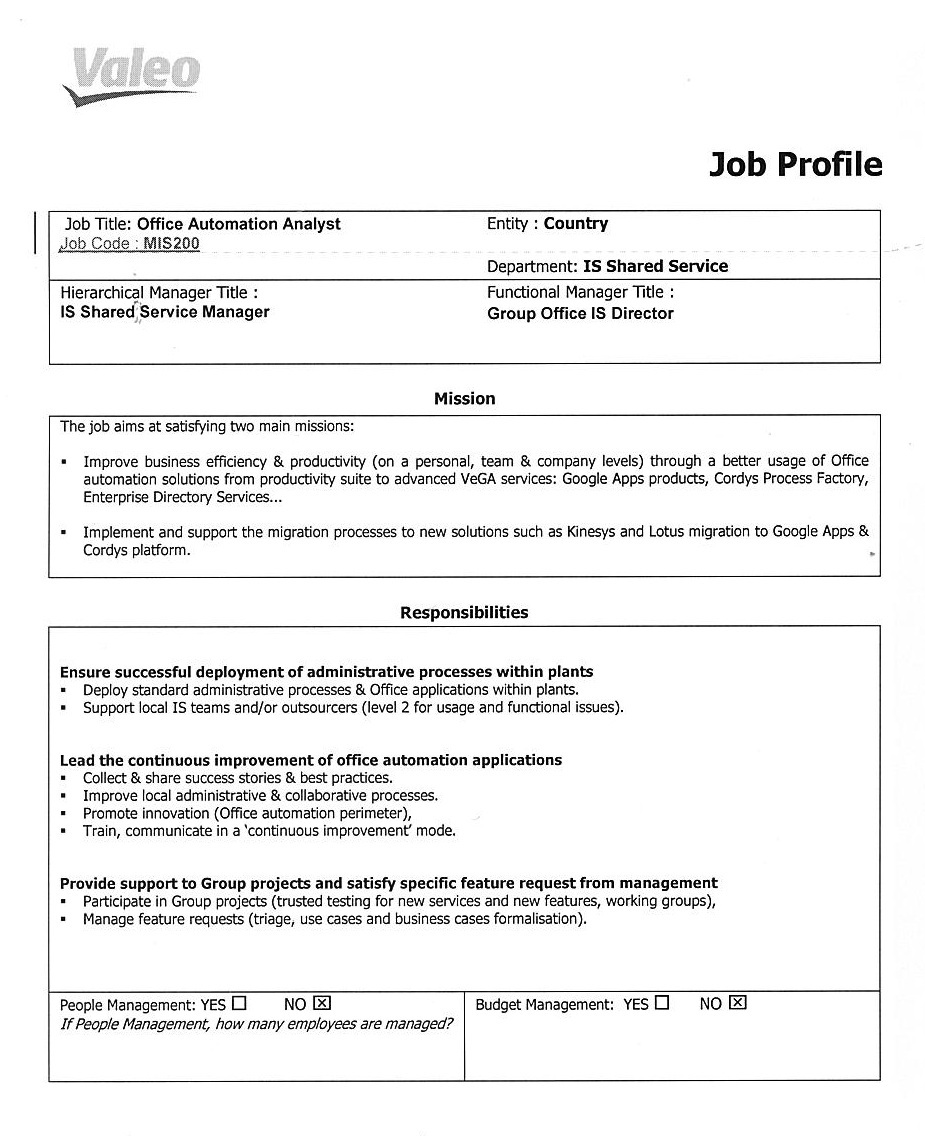
\includegraphics[height=22cm]{job_profil.jpg}
	\caption{Fiche de poste}\label{image.jobprofil} 
\end{figure} 

\clearpage


\chapter{METIS, un projet de recherche}

\section{Description du Projet de Recherche}

\textbf{Source : \url{http://metis.deltacad.fr/}}

Le projet \textbf{METIS} est un projet de recherche collaboratif impliquant deux industriels (\textbf{DeltaCAD} et \textbf{IFPEN}) et 4 laboratoires universitaires (\textbf{AMPT}, \textbf{ECN}, \textbf{UTC} et \textbf{UTT}). Ce projet est prévu pour durée de 3 ans et a débuté en octobre 2012. Le projet est subventionné par l'\textbf{ANR}, Agence Nationale de la Recherche (\url{http://www.agence-nationale-recherche.fr/}), dans le cadre du programme \textit{Modèle Numérique 2012}.

Ce projet s’intègre dans le domaine de la rétro-conception (ou \textit{Reverse Engineering} en anglais).
 
Aujourd’hui, la rétro-conception est largement utilisée dans l’industrie manufacturière afin de capitaliser des connaissances qui ne l’ont pas été jusque-là et qui deviennent aujourd’hui cruciales pour faire évoluer ses produits.
Les applications sont diverses, comme par exemple, la rétro-conception de produits existants en vue d’en modifier/combiner des composantes (cas d’IFP Energies nouvelles par exemple, qui fait de la rétro-conception de moteurs) ou alors la maintenance des produits mécaniques à très longue durée de vie (avions, navires, centrales nucléaires, plateformes pétrolières, trains…), lorsqu’il faut reconcevoir et refabriquer un composant autrefois produit soit en interne mais dont le personnel a quitté la société ou soit par un sous-traitant aujourd’hui disparu.
                                
De manière générale, les solutions commerciales présentes actuellement sur le marché proposent d’extraire les informations géométriques de l’objet afin de le reconcevoir (RAPIDFORM XOR d’Inus Technology par exemple).
Il existe également dans la littérature scientifique des approches traitant de la rétro-conception de composants ou de petits ensembles. Dans ce cas, la géométrie de l’objet est souvent obtenue par numérisation 3D ou mesure. La surface de l’objet est ainsi échantillonnée par un nuage de points et/ou un maillage surfacique. Aujourd’hui, c’est l’analyse de cette géométrie à travers un filtre de connaissances métier qui permet de retrouver les intentions initiales de conception et d’en assurer la rétro-conception.
 
Le projet \textbf{METIS} vise, quant à lui, à proposer des solutions pour la rétro-conception de grands ensembles mécaniques complexes (par le nombre de pièces et/ou leur taille) tels que des moteurs, des véhicules (ces problématiques étant au cœur des travaux d’IFP Energies nouvelles) par exemple. Dans le cadre de ces ensembles, il est délicat et peu efficace de numériser intégralement la géométrie. Par exemple, pour une automobile, relever le nuage de points de l’ensemble des pièces qui la composent serait, sinon impossible, extrêmement fastidieux. En effet, il faudrait, pour cela, démonter l’intégralité de la voiture et numériser les pièces une à une, manuellement : les systèmes de numérisation 3D automatiques de pièces dont on ne possède pas la CAO (impossibilité de faire une gamme automatique) sont très limités dès qu’il s’agit de pièces de formes complexes, la numérisation des pièces de la voiture devrait donc se faire majoritairement manuellement.
 
L’hypothèse principale portée par le projet \textbf{METIS} est que, pour la rétro-conception d’un grand ensemble mécanique complexe, les informations purement géométriques sont insuffisantes. METIS vise à proposer une solution pour intégrer l’ensemble des informations (y compris les informations géométriques) disponibles sur l’ensemble mécanique étudié afin de les traiter et d’en extraire une maquette numérique.
 
Il s’agit donc de développer des méthodologies ainsi que les outils associés qui permettront à un utilisateur de créer et maintenir dans le temps une maquette numérique sémantiquement riche et intégrant les connaissances liées à l’ensemble mécanique considéré. Cette maquette sera obtenue à partir d’informations hétérogènes, parfois incomplètes, telles que des images, des plans 2D, des nuages de points issus de numérisations 3D, des croquis, des photographies, des rapports de maintenance, des résultats de calculs…, voire même une ancienne version de la maquette numérique.

\section{Contexte scientifique}

L’objectif de METIS est de permettre la création ou la mise à jour de la maquette numérique d’un ensemble mécanique complexe existant (ex : un moteur). A partir du grand ensemble de données hétérogènes et d’une bibliothèque de composants appartenant à un domaine (composants mécaniques, mobilier, tubes, outillages, architecture), l’outil METIS permettra de déterminer automatiquement le type et le nombre de composants présents dans un ensemble mécanique complexe. Il permettra aussi de déterminer la position et l’orientation de chaque composant. Une fois que l’intégralité de la nomenclature du produit aura été déterminée et qu’une matrice de position aura été associée à chacun des composants de cette nomenclature, l’outil METIS permettra de générer la maquette numérique de ce grand ensemble mécanique. Les fonctions principales de cet environnement de rétro-conception sont les suivantes :


\begin{enumerate}
  \item Acquisition, traitement et intégration de grand volume de données, géométriques ou non, spatialement localisées : les données recueillies seront d’une telle hétérogénéité (nuages de points 3D, photographie, référence catalogue, résultats de calcul, schémas de maintenance, ancienne version de la maquette numérique etc.) qu’il faudra développer une méthodologie de triage et de mise en correspondance et de référencement innovante. Nous pourrons proposer des méta-modèles basés sur des évolutions des formalismes de cartes cognitives, de réseaux sémantiques par exemple. \\
  
  \item Méthode d’identification de composants métier dans un ensemble de données hétérogènes : il s’agira de créer d’une bibliothèque de composants caractérisés par des éléments clés (signature) permettant leur identification dans un grand volume de données. L’apport scientifique est  ici de trouver un moyen de « signer » des composants complexes et de stocker ces signatures. Elles seront établies en géométrie 2D (photographie, plan, croquis), en géométrie 3D (nuage de points) et sous toute autre forme qui pourrait être pertinente (signatures non géométriques). Cette bibliothèque permettra d’identifier, dans les données acquises précédemment, des éléments de maquette numérique associés à une signature particulière.\\
  
\clearpage

  \item Recherche, dans le grand volume de données, de la nomenclature du produit étudié ainsi que des matrices de position associées : dés qu’un composant est reconnu (identification de sa signature), le premier apport scientifique sera de le caractériser dans ses dimensions, sa position, son orientation etc. à l’aide de données géométriques et non géométriques recueillies directement dans l’ensemble de données mais aussi à l’aide de connaissances connues a priori sur le composant (ex : dépouilles si composant forgé etc.). Le second apport scientifique sera la gestion des différents niveaux de décomposition systémique lors du déroulement de METIS. En effet, l’analyse de rétro-conception peut aussi bien porter sur un système complet (ex : voiture), un sous-système (ex : ensemble moteur) ou un composant élémentaire (ex : alternateur). Les signatures et leur reconnaissance devront alors être modélisées et gérées dans ces différents niveaux systémiques qui doivent rester cohérent au fil du temps et selon la granularité de l’analyse.\\
  
  \item Génération ou modification de la maquette numérique : dés la nomenclature connue, les modèles CAO paramétrés métier associés aux différents composants pourront être :
assemblés au sein du modèle géométrique du grand ensemble étudié.
modifiés par corrélation des modèles géométriques originels et des nouveaux paramètres géométriques identifiés ou par échanges d’une partie des composants de la maquette numérique originelle. L’apport scientifique réside dans la mise en œuvre d’algorithmes et de stratégies relatifs à la manipulation de la maquette numérique soit pour la gestion de la nomenclature (ex : filtre de composants, etc.) soit pour la gestion des éléments géométriques eux-mêmes (ex : déformation, ajout sémantique, dimensionnement, etc\ldots).\\
\end{enumerate}

\clearpage


\chapter{Le Cloud Computing}
\section{Qu'est ce que le Cloud Computing ?}

Le Cloud Computing ( ou ``Informatique dans les Nuages" en français) est un secteur de l'informatique en plein essor depuis quelques années.
Un de ses concepts fondateurs est la mise à disposition de technologies et services à la demande : \textit{``as a service"}.

La vision est d'offrir aux utilisateurs un service à la demande où celui ci ne paie que sa consommation (une analogie avec le service  d'eau, d'électricité, de gaz peut être établie en France contrairement à certaines villes comme Moscou où l'on paie un forfait à l'année pour le gaz en illimité).

Cette technologie est actuellement en plein essor. De nombreux acteurs misent sur cette nouvelle manière d'envisager l'informatique. Parmi lesquels nous retrouvons Google, Amazon, Microsoft, IBM, SalesForce, DropBox, Apple, ... Des technologies à la fois orientés grand public et entreprises sont développés. Je citerai par exemple le Google Drive et Google Apps qui sont en fonction chez Valeo.\\
De plus en plus de domaines sont à présent concernés : \emph{Emails, Traitement de Texte, Stockage de Données, Jeux ...}

Le ``Cloud" se base sur une faculté native à s'adapter de manière élastique aux besoins des utilisateurs. À fournir des services en temps réel ou en ponctuel, à forte ou faible capacité (en terme de débit de connexion et de capacité de calcul). Ce sont tous ces facteurs qui font du ``Cloud" une valeur montante de l'informatique.

 \begin{figure}[H]
    \centering
    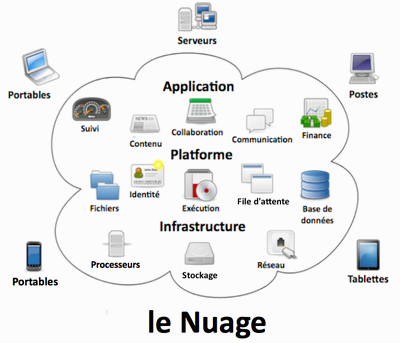
\includegraphics[height=9cm]{cloud.png}
	\caption{Représentation du Cloud - \cite{image.cloud.source} }\label{image.cloud} 
\end{figure}

\section{IaaS vs PaaS vs SaaS vs STaaS}

Quand on parle d'un ``Service Cloud", il y a trois catégories possibles :

\begin{itemize}
	\item \textbf{Infrastructure as a Service (IaaS):}\\ 
	
	Dans ce type d'architecture, \emph{\textbf{le fournisseur}} du service s'engage à livrer et maintenir le serveur, son OS (virtuel ou non), le stockage et le réseau nécessaire.\\
			
	Il reste à la charge \emph{\textbf{du client}} la gestion de la \textit{plateforme} et des diverses applications qui fonctionnent sur cette dernière, les bases de données et les différents logiciels installés.\\
	
	Ce type de service est grandement utile aux entreprises désireuses de revendre des services Cloud type Saas ou Paas de louer des infrastructures hautement flexibles. Pour ne citer que quelques exemples voici quelques fournisseurs de IaaS :\emph{ Cloud Power, DotRiver, Amazon EC2, Windows Azure, Rackspace,~...}\\
			\vspace{8mm}
			
		
	\item \textbf{Platform as a Service (PaaS):}\\
	
	Dans ce type d'architecture, \emph{\textbf{le fournisseur}} du service s'engage à livrer et maintenir tout ce qui compose l'IaaS. A celà s'ajoute en plus la partie plateforme cloud, les bases de données, et les logiciels nécessaires au fonctionnement de la plateforme ou de l'administration du serveur.\\
			
	Il ne reste à la charge \emph{\textbf{du client}} que la gestion des \textit{applications} (et leur dévelopement au besoin) sur la plateforme cloud fournie.\\

Ce type de service est généralement destiné aux utilisateurs finaux, et sont utilisés par de plus en plus de personnes ayant des besoins spécifiques et ne voulant déployer de gros moyens à chaque nouveau projet (petit ou grand) : On retrouvera dans les plateformes : \emph{Force.com pour SalesForce, Google AppEngine, Cordys Process Factory} (sur lequel j'ai travaillé), Microsoft Azure \emph{...}\\
			\vspace{8mm}
	
	
	\item \textbf{Software as a Service (SaaS):}\\
	
	Le Software as a service (SaaS) est l’ultime modèle de Cloud, où \textbf{le fournisseur} Cloud 
maintient absolument tout et developpe les applications.\\
	
	Le \textbf{client} lui est simple ``\emph{utilisateur}" des applications.\\
	
	Ainsi nous retrouvons les applications clouds suivantes en tant que SaaS: \emph{Google Document, Google SpreadSheet, ... }\\
			\vspace{8mm}

\item \textbf{Storage as a Service (STaaS):}\\

 Très similaire au SaaS, seulement cette fois-ci le client ne veut pas une application mais un espace de stockage.\\
 
 \emph{Services Connus : Google Drive, Dropbox, iCloud, Microsoft Skydrive,} ...

\end{itemize}
			\vspace{2cm}
 
\begin{figure}[H]
    \centering
    \includegraphics[height=14cm]{aas.png}
	\caption{IaaS vs PaaS vs SaaS - 	\cite{image.aas.source}}\label{image.aas} 

\end{figure}
\clearpage

\chapter{Cordys Process Factory}
%https://www.tpfcloud.com/cordys/uc/webapps/onlinehelp/tasks/creating_an_application.htm#task_4424A9209E894BBE966E2963F1BCBED8
\section*{Avant Propos}

Cordys Process Factory fut un des points centraux de mon stage. Comme il ne m'est pas possible de décrire avec précision chacun de ses points, j'ai choisi de détailler mon travail dans la partie qui pour moi présente le plus d'intérêt. 

Cordys Process Factory étant une plateforme propriétaire et bénéficiant d'une interface de \emph{développement au clic}, je m'attacherai à en décrire avec minutie le fonctionnement, tous les outils qui sont mis à disposition sur la plateforme et leurs interactions avec autant que possible des références au travail que j'ai pu mené à Valeo.

\section{Une plateforme Applicative ``Cloud"}

\subsection{Qu'est ce que Cordys Process Factory ?}

Cordys Process Factory est un service orientée \textit{Cloud Computing}. Cette solution Cloud est de type PaaS : Plateforme as a Service. Elle permet de développer des applications répondant à une demande de \textit{``Business Workflow"}. C'est un besoin critique dans un environnement comme celui de Valeo. 

Les utilisateurs classiques, tout comme les développeurs, peuvent utiliser la plateforme pour \textbf{composer} des applications de manière simple et rapide en ayant reçu une brève formation sur l'outil(\textbf{sans connaissances en programmation informatique} ou presque). \\
La plateforme est également capable de s'interfacer avec les différents systèmes existants et les \textit{Cloud Services} actuellement en fonction dans l'entreprise. Un point qui fut très important dans le choix de cette plateforme.

\clearpage

\subsection{Lotus Notes vs Cordys Process Factory}

Lotus Notes (solution logicielle développée par \textbf{IBM}) et Cordys Process Factory (solution Cloud développée \textbf{Open~Text}) ont un objectif commun : proposer une réponse au  besoin de ``\textit{Business Processing}" au sein d'une entreprise.

Cependant elles diffèrent sur l'architecture (serveurs et réseau) nécessaire à son fonctionnement :

\begin{itemize}
		\item Lotus Notes se base sur une architecture type logiciel Client / logiciel Serveur, les serveurs sont inter-connectés entre eux et ``\textit{répliquent}" certaines de leur données à intervalle de temps régulier. Ce fonctionnement est coûteux , il demande une infrastructure imposante ainsi qu'une administration au jour le jour. \\
		Plus gênant, comme il est difficile d'avoir une vue d'ensemble du système actuel, la quantité d'application dupliquée ne cesse d'augmenter, ce qui induit des coûts de fonctionnement de plus en plus élevés.\\

	\item Cordys Process Factory propose une réponse orientée ``\textit{Cloud Computing}" à ces problématiques, nous pouvons donc faire \textit{abstraction} de l'architecture réseau et serveur nécessaire à son fonctionnement (gérée par le fournisseur du service). La plateforme est accessible via un navigateur web, nul besoin de paramétrer son ordinateur ou d'installer un quelconque logiciel.\\
	Le choix de Cordys Process Factory est donc cohérent avec la politique actuelle du groupe Valeo qui cherche à \emph{externaliser} la gestion de la partie infrastructure et l'administration des diverses solutions informatiques.\\
	\end{itemize}


\subsection{Le contexte dans lequel s'insère Cordys Process Factory}

Valeo a fait le choix de se baser en grande partie sur la suite Google Apps pour un maximum de services et besoins bureautiques. Ainsi nous utilisons de manière non exclusive: 

	\begin{itemize}
		\item Gmail
		\item Google Drive
		\item Google Apps (SpreadSheet, Docs, Presentation, Scripts, Sites)
		\item Google Agenda 
		\item Google AppEngine
	\end{itemize}

En complément nous utilisons un LDAP, commun à tous les sites Valeo du monde, interfacé avec la suite applicative de \textbf{Google}. Valeo appelle cet ensemble de systèmes inter-opérants  : VeGA \textit{(Valeo empowered by Google Apps)}.

\clearpage

\textbf{Et \textit{Cordys Process Factory} dans tout ça ?}

Fort de sa position de partenaire \emph{Google Entreprise}, Cordys Process Factory permet une inter-connection aux services Google Apps  et le LDAP de Valeo : \textit{l'Entreprise Directory}.\\
Ainsi les \textit{Businness Process} et \textit{Businness Workflows} peuvent s'appuyer sur les services et applications déjà en place chez Valeo afin de réduire les coûts de mise en place et de développement.

\clearpage
\section{Présentation du fonctionnement de la Plateforme de Service}

\subsection{Architecture de la plateforme }

La plateforme Cordys fonctionne en trois mandants.
\vspace{4mm}
\begin{itemize}
	\item Mandant de Production
	\item Mandant de Test (ou Acceptance)
	\item Mandant de Développement
\end{itemize}
\vspace{4mm}

Les utilisateurs ``classiques" n'ont accès qu'au mandant de production, c'est ce dernier le plus important: il contient les données Business de l'entreprise.

Les développeurs d'applications sur la plateforme Cordys peuvent accéder à l'environnement de test qui est une réplication complète de l'environnement de production (en terme de services et logiciels en place). Il est essentiel de tester une application dans ce mandant avant de la déployer en production de sorte à vérifier la compatibilité avec le futur environnement. Cette étape est absolument nécessaire du fait de l'impossibilité d'altération ou suppression des données Business et stratégiques dans ce mandant.

Concernant le mandant de développement, c'est le seul mandant qui n'est pas rattaché aux services Valeo, Google et LDAP. Ce dernier est uniquement là pour développer et tester les applications de manière succincte  avant de les soumettre à validation.


Nous suivons donc un Workflow de développement de type DTAP : Development, Testing, Acceptance and Production : 

\begin{enumerate}
	\item Une fois que le développeur pense que l'application est prête, elle est copiée dans l'environnement de test pour vérifier qu'elle fonctionne comme attendue.\\
	Les tests ne sont pas normalisés comme ils devraient l'être dans un Workflow de type DTAP. Il appartient à chaque développeur de s'assurer du fonctionnement de son application.\\
	 \item Une fois les tests positifs, l'application est passée en revue avec le ``Business Owner" de la future application (celui qui sera responsable de cette application et des données Business qui y transiterons). Ce dernier vérifiera que l'application correspond bien à son besoin. \\
	 \item Après l'acceptation de l'application par le ``Business Owner", l'application est déployée en production et rendue accéssible.
\end{enumerate}

 \begin{figure}[H]
    \centering
    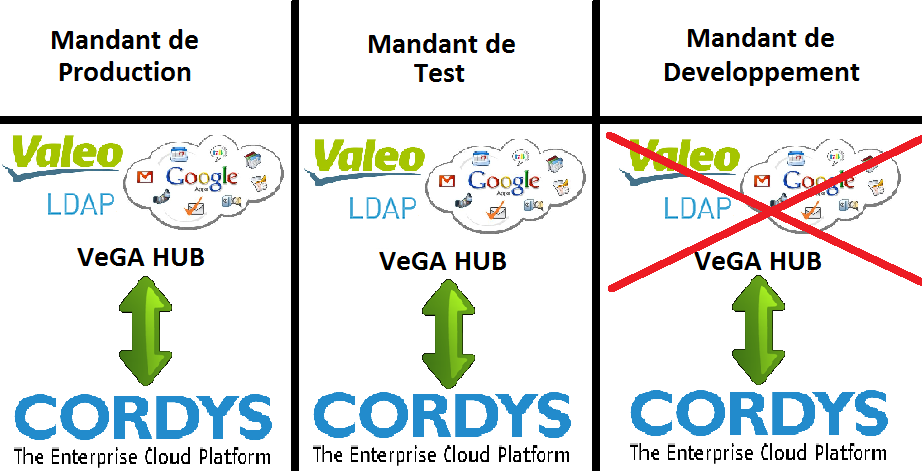
\includegraphics[height=9.25cm]{architecture_Cordys.png}
	\caption{\textit{Schéma de l'architecture Cordys chez Valeo}}\label{image.architectureCordys} 
\end{figure}

\clearpage

\subsection{Présentation de l'interface standard d'une application}


L'interface d'une application Cordys est relativement identique quelque soit l'application.\\
Ainsi, quel que soit l'application, deux onglets sont systématiquement disponibles : \textit{My Page \& Setup}.
Le nom de l'application se situe en haut à gauche, se qui constitue un bon repère visuel.\\
En plus de celà, un menu déroulant ``Change Application", permet d'afficher la liste entière des applications auxquelles vous avez le droit d'accéder.

 \begin{figure}[H]
    \centering
    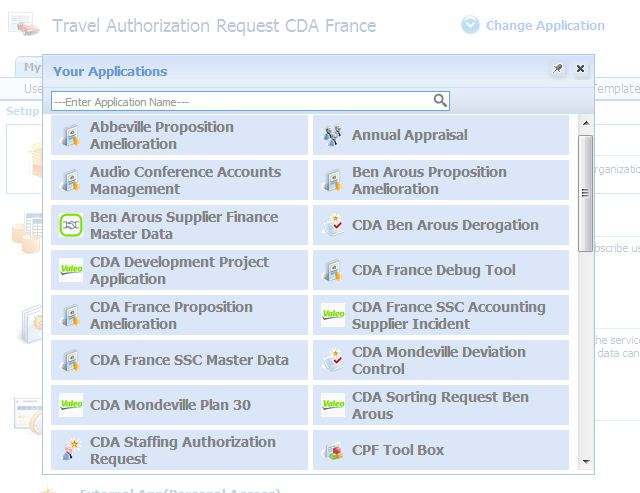
\includegraphics[height=6cm]{cordysChangeApplication.jpg}
	\caption{\textit{Interface Standard d'une application Cordys - Menu ``Change Application"}}\label{image.CordysChangeApplication} 
\end{figure}

\subsubsection{L'onglet My Page}

La vue par défaut d'une application est l'onglet: ``My Page". Il regroupe les dernières données relatives à l'utilisateur.

 \begin{figure}[H]
    \centering
    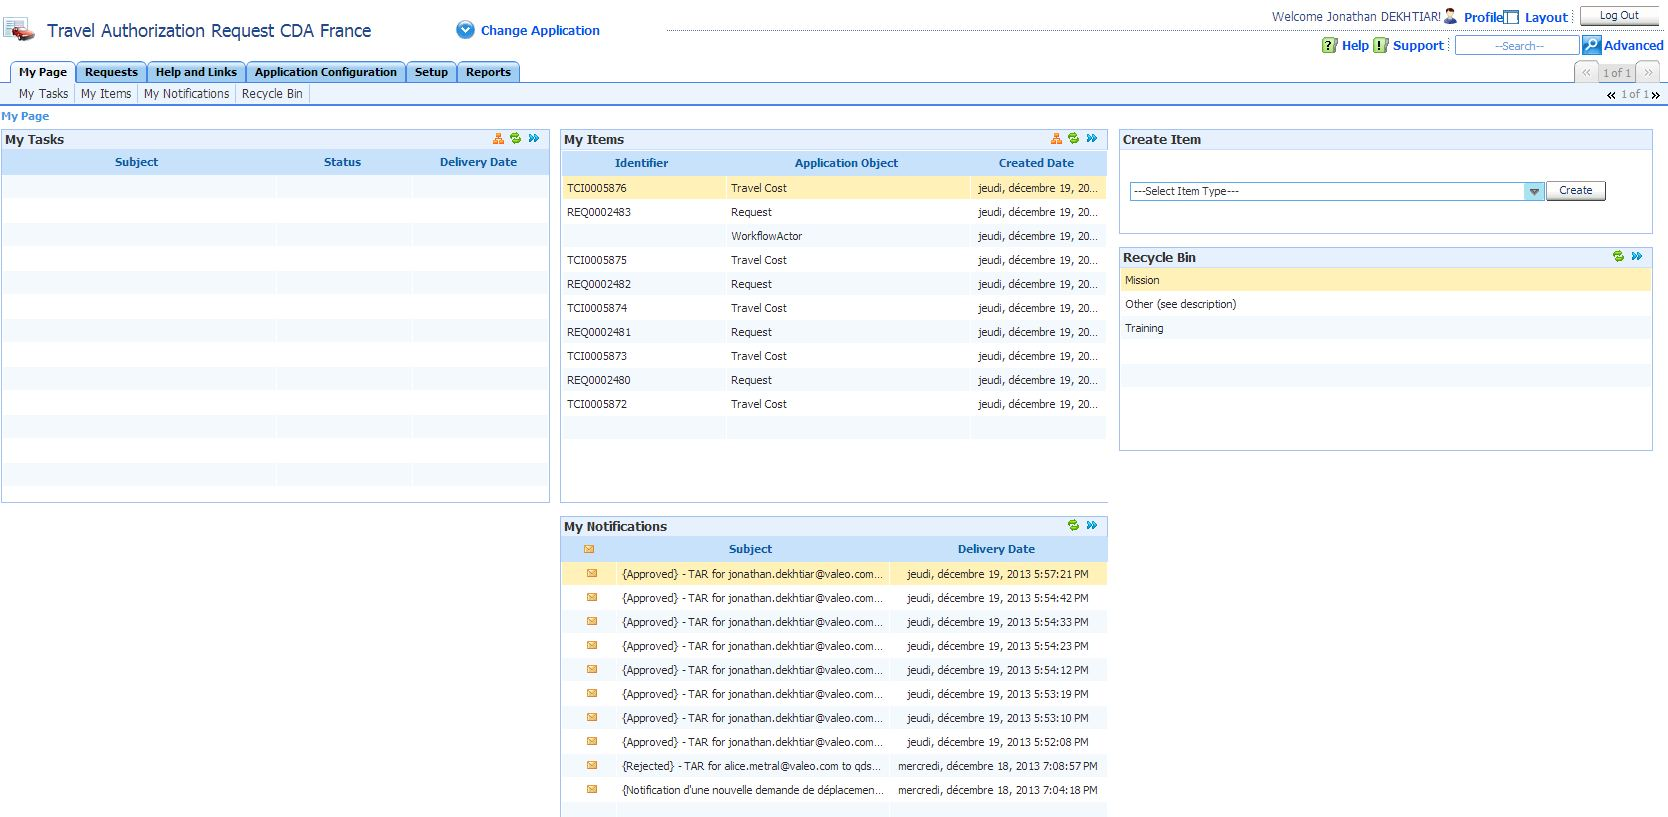
\includegraphics[height=8cm]{cordysMyPage.jpg}
	\caption{\textit{Interface Standard d'une application Cordys - Onglet ``My Page"}}\label{image.CordysMyPage} 
\end{figure}

\subsubsection{L'onglet Setup}

L'onglet Setup varie en fonction des droits d'accès. Un utilisateur aura accès uniquement à la personnalisation de son interface (de manière assez restreinte) et l'administrateur pourra, lui, accéder à plusieurs rubriques permettant l'import de données dans l'application, l'analyse des processus en cours d'éxécution, les tâches actuellement en attentes (et les réaffecter si nécessaire), la liste des utilisateurs de l'application et leurs droits respectifs (en lecture et en modification), ainsi que d'autres fonctions moins utiles comme les modèles d'emails ou l'état des nombres auto-incrémentés.

 \begin{figure}[H]
    \centering
    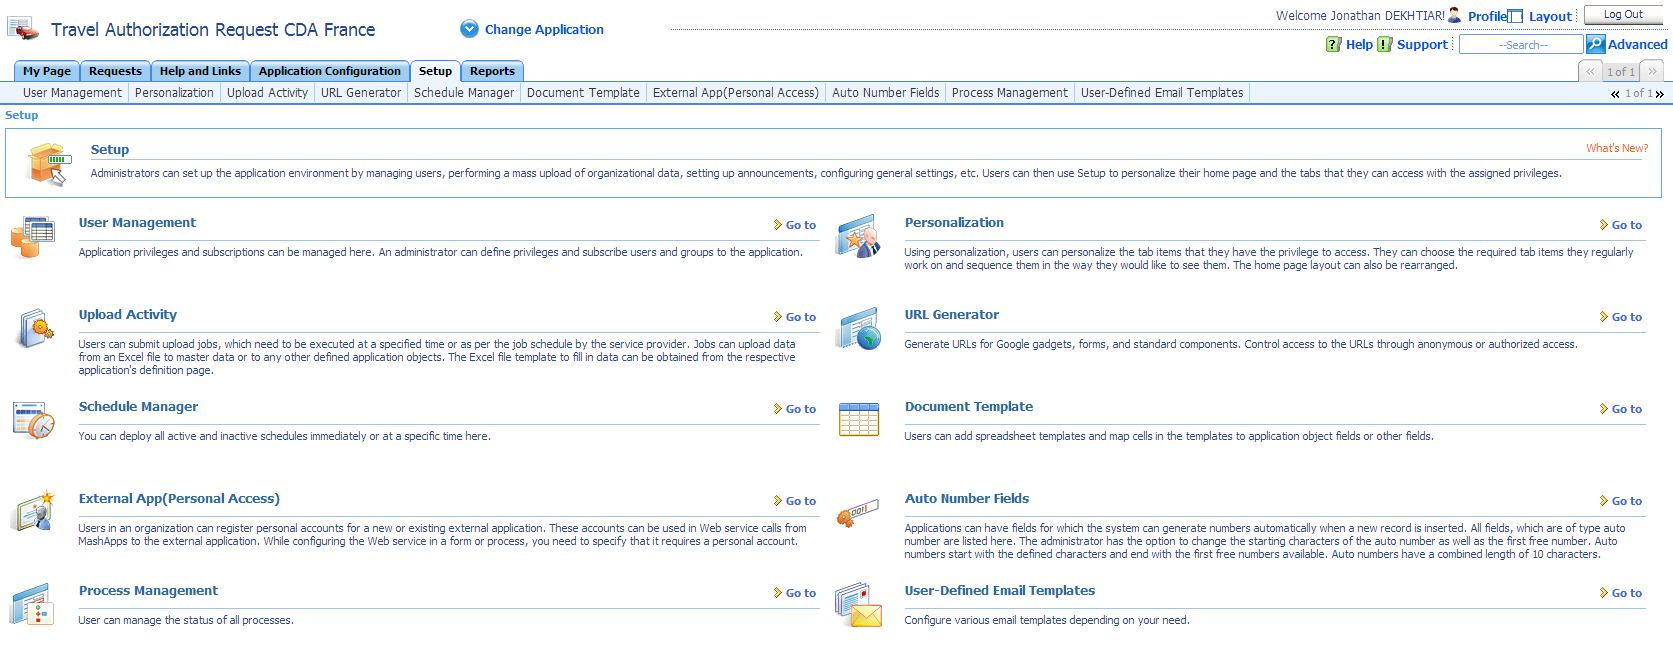
\includegraphics[height=7cm]{cordysSetupAdmin.jpg}
	\caption{\textit{Interface Standard d'une application Cordys - Onglet ``Setup" - Vue Administrateur}}\label{image.CordysSetupAdmin} 
\end{figure}

 \begin{figure}[H]
    \centering
    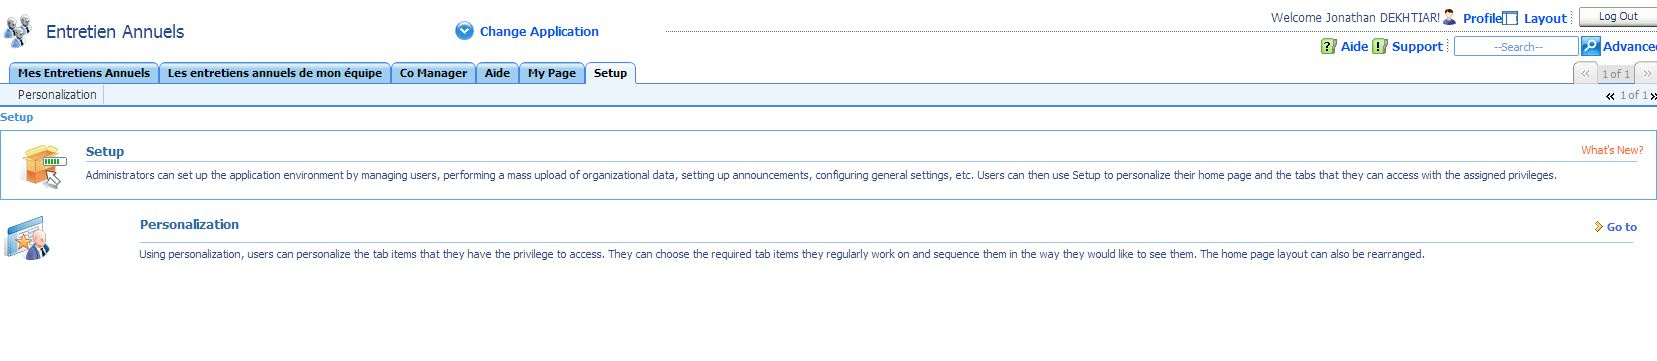
\includegraphics[height=3.8cm]{cordysSetupUser.jpg}
	\caption{\textit{Interface Standard d'une application Cordys - Onglet ``Setup" - Vue Utilisateur}}\label{image.CordysSetupUser} 
\end{figure}

\clearpage

\subsubsection{L'onglet Report}

L'onglet Report est automatiquement disponible pour chaque application, cependant l'administrateur peut choisir ou non de le faire apparaitre dans l'application et/ou de le rendre disponible uniquement pour une partie des utilisateurs ou pour tout le monde en modifiant les droits d'accès.

Les Reports sont à ``paramétrer" en développement pour qu'ils apparaissent en production de manière systématique. Sinon ``\emph{l'instant Report}" permet d'extraire des données de manière rapide et flexible. Il est cependant plus long à effectuer qu'un Report automatique et nécessite la connaissance du nom des champs que l'on veut extraire.

 \begin{figure}[H]
    \centering
    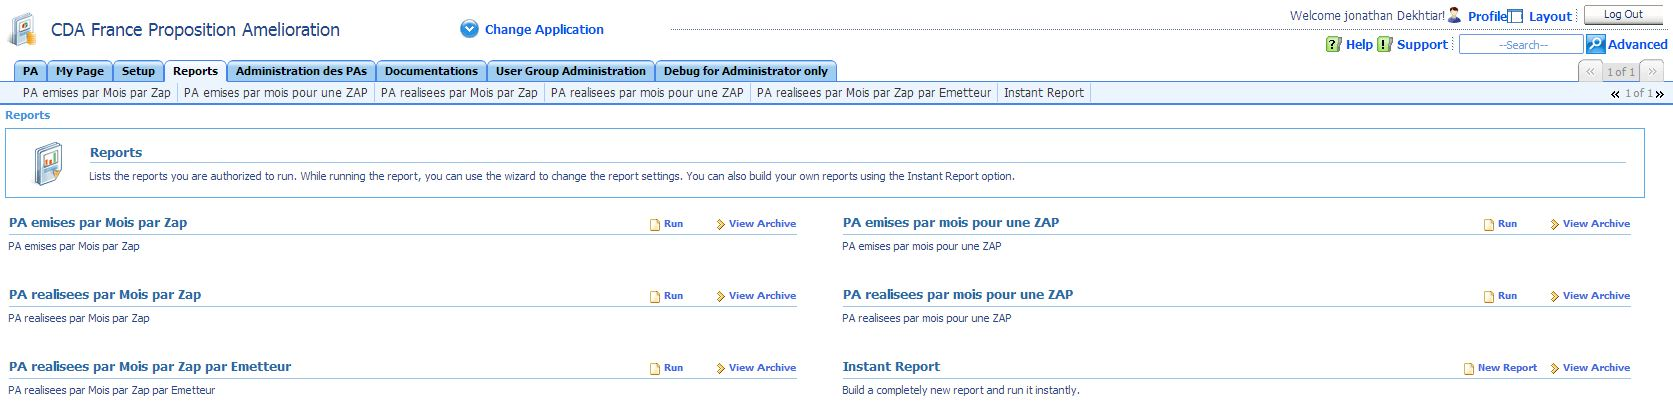
\includegraphics[height=3.8cm]{cordysReports.jpg}
	\caption{\textit{Interface Standard d'une application Cordys - Onglet ``Report"}}\label{image.CordysReports} 
\end{figure}

\clearpage

\subsection{Présentation de l'interface developpeur de Cordys}

\subsubsection{La page d'accueil de la plateforme de développement}

La page d'accueil de la plateforme de développement est assez sobre, on y retrouve les différentes sections sur la gauche et une vue ``graphique" au centre expliquant à quoi sert cet onglet. Toujours dans l'optique de permettre à un utilisateur, sans bagage informatique, de pouvoir mettre en place simplement et rapidement en place une application.

 \begin{figure}[H]
    \centering
    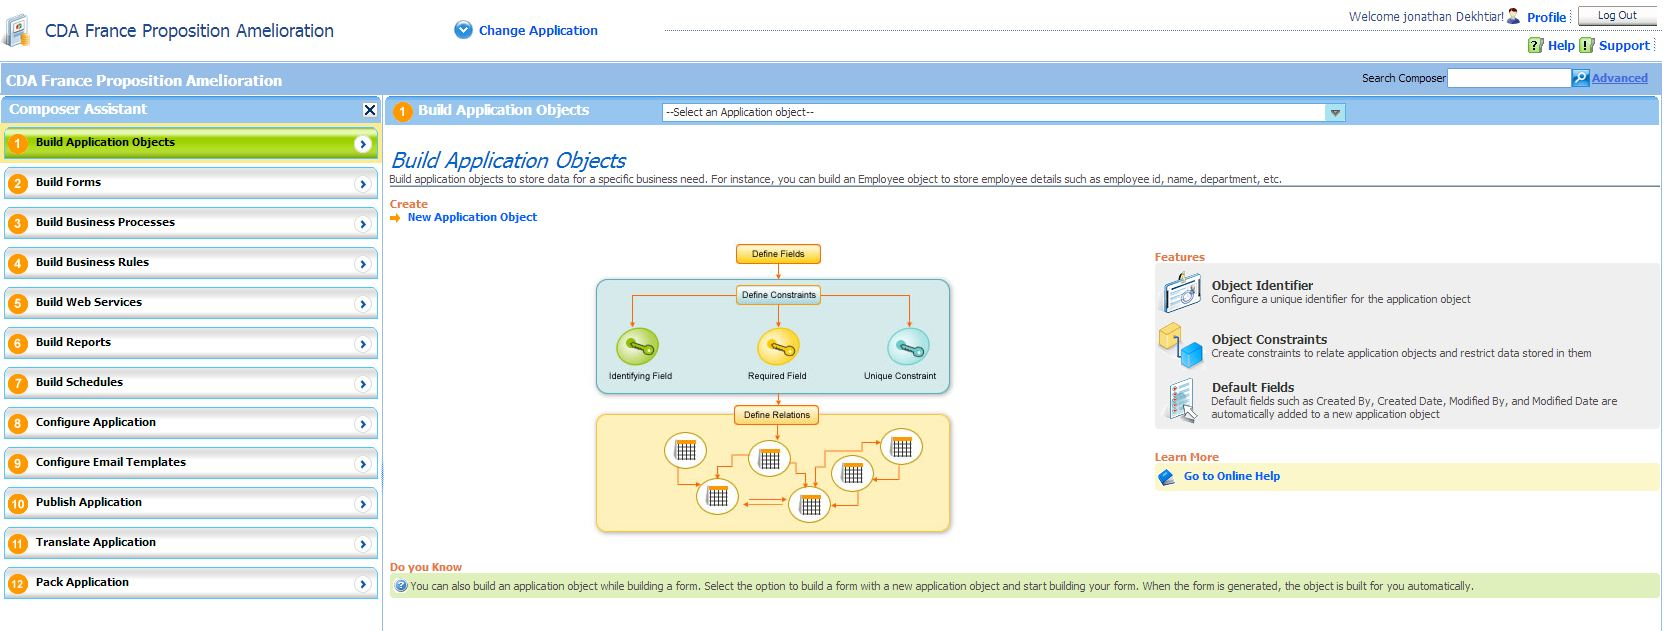
\includegraphics[height=6.9cm]{cordysDevHome.jpg}
	\caption{\textit{Interface de développement de Cordys - Page D'accueil}}\label{image.CordysDevHome} 
\end{figure}

\subsubsection{L'onglet ``Application Object"}

Un \emph{Application Object} est l'équivalent de ce qu'on appelle en programmation orientée objet : \textbf{un objet}.\\
Ces objets sont la base de l'application, ils sont à définir selon les besoins et donc selon le cahier des charges qui a été établi au préalable.\\
Des diagrammes UML sont donc à prévoir sur les applications lors de la définition du projet.

Les \emph{Application Objects} permettent de stocker les données relatives à l'entreprise. Par exemple, les dépenses de l'entreprise dans une application dédiée à la validation des factures ou au remboursement des frais des employés.

Afin de stocker des données dans un \emph{Application Object}, il est nécessaire d'ajouter donc des champs relatifs à l'utilisation (Exemple: FactureID, UserName, ApproverName, ...).

Lors de la création de l'\emph{Application Object}, il est possible de définir la clé primaire, des index afin de faciliter et accélerer la recherche et des contraintes (sur un ou plusieurs champs).

Tous les \emph{Application Object} sont stockés dans l' \emph{``Application Object Repository"}. Il est ainsi possible de les modifier, et de les supprimer par l'intermédiaire de ce répertoire.

 \begin{figure}[H]
    \centering
    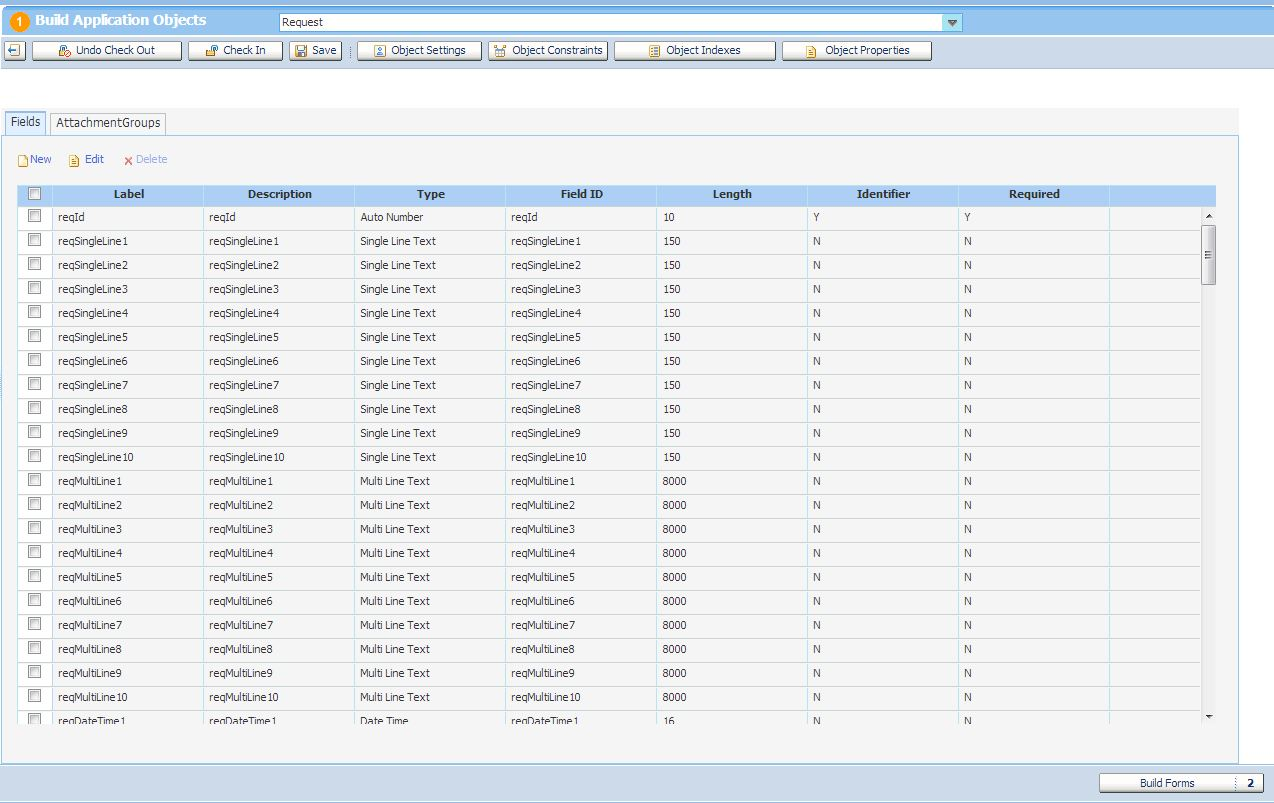
\includegraphics[height=11cm]{cordysDevAOForm.jpg}
	\caption{\textit{Interface de développement de Cordys - Interface de définition des Application Object}}\label{image.CordysDevAOForm} 
\end{figure}

\clearpage

\subsubsection{L'onglet ``Forms"}

Une fois un \emph{Application Object} défini, il est possible de créer un ou plusieurs formulaires de manière à permettre l'instanciation de ces objets. Tous les champs relatifs à cet \emph{Application Object} sont automatiquement ajoutés au formulaire, charge au développeur de choisir s'il désire tous les garder et de les agencer à sa convenance.\\
Il est également possible de créer un formulaire sans le rattacher à un \emph{Application Object}. Dans ce cas, il est impossible de sauvegarder les informations entrées dans ce formulaire et celles affichées par les différents Web-Services appelés.

Différents outils sont à disposition afin de mettre en place le formulaire répondant exactement aux attentes: 

\begin{itemize}\itemsep5pt
	\item \textbf{Les Types de Sections: }Il possible de créer différent types de section pour organiser les champs du formulaire. Ces sections portent le nom de : ``Group Box", ``Grid", et  ``Tab sections". Il est également possible de créer une section pour attacher un ou plusieurs fichiers et des éventuels commentaires.
		
	\item \textbf{Les types de Champs: }De nombreux types de champs sont à disposition des développeurs, le choix dépend alors du type d'information qui y sera stocké.
	
	\item \textbf{Le ``Repertoire" de Web Services: }Tous les Web services de l'application sont stockés dans un répertoire. Il est ainsi possible d'ajouter des Web Services, basés sur des Application Objects et Business Process, à un formulaire directement depuis ce répertoire. Il est également possible d'ajouter des Web Services ``externes" SOAP ou REST.
	
	\item \textbf{Les Paramètres de Formulaire: }Une des sources de flexibilité dans la création des formulaires vient de ce qu'on appel les ``Form Parameters" ou en Français : Les Paramètres de Formulaire. Ils permettent de définir quels champs seront les entrées ou les sorties d'un ou plusieurs Web Services.
	
	\item \textbf{Design adaptatif: }Les formulaires peuvent être créés de manière ``flexible" et s'adapter à la taille de la fenêtre ou du design établi (\textit{Responsive Design}). Les Sections, champs et Web Services peuvent être placés de manière quelconque dans le formulaire.
			
	\item \textbf{Les champs de type ``Lookup": }Il est possible de paramétrer des champs pour les associer à un ``\emph{lookup}". Cela leur permettra de \textbf{sélectionner} des données relatives à des Application Objects ou aux Utilisateurs (Groupes, Fonction, Email  ...).

	\item \textbf{Les règles de Formulaire: }Il est possible de définir des conditions qui vont modifier le comportement d'un formulaire en utilisant ce qu'on appelle une ``Règle de Formulaire". Il est ainsi possible d'assigner des valeurs, afficher des messages, cacher ou forcer l'affichage, bloquer ou débloquer un champs, une section.
	
	\item \textbf{Les vues: }Il est possible de créer des vues de manière à trier les données pour les formulaire de type tableau ou ``Grid" en anglais.
	
	\item \textbf{L'éditeur de Script: }Ce dernier module permet aux développeurs plus chevronnés d'avoir un contrôle total de leur formulaire avec l'aide du Javascript et un petite sur-couche \textit{made in Cordys}.

\end{itemize}

En dehors des fonctions citées plus haut, un système de versionnement est en place et permet d'afficher les dix dernières révisions de l'objet ou du formulaire via un système de ``Check In" / ``Check Out"  dans le but d'améliorer l'efficience et de réduire la maintenance. Il est également possible de modifier le formulaire de sauvegarder et de ne finalement rendre les modifications effectives que plusieurs jours après en effectuant le ``Check In" au bon moment.

Il est possible de prévisualiser le formulaire pendant son édition. Cette fonction permet de vérifier le bon comportement pendant l'exécution (en particulier les scripts et règles de formulaires).
\vspace{8mm}

\begin{figure}[H]
    \centering
    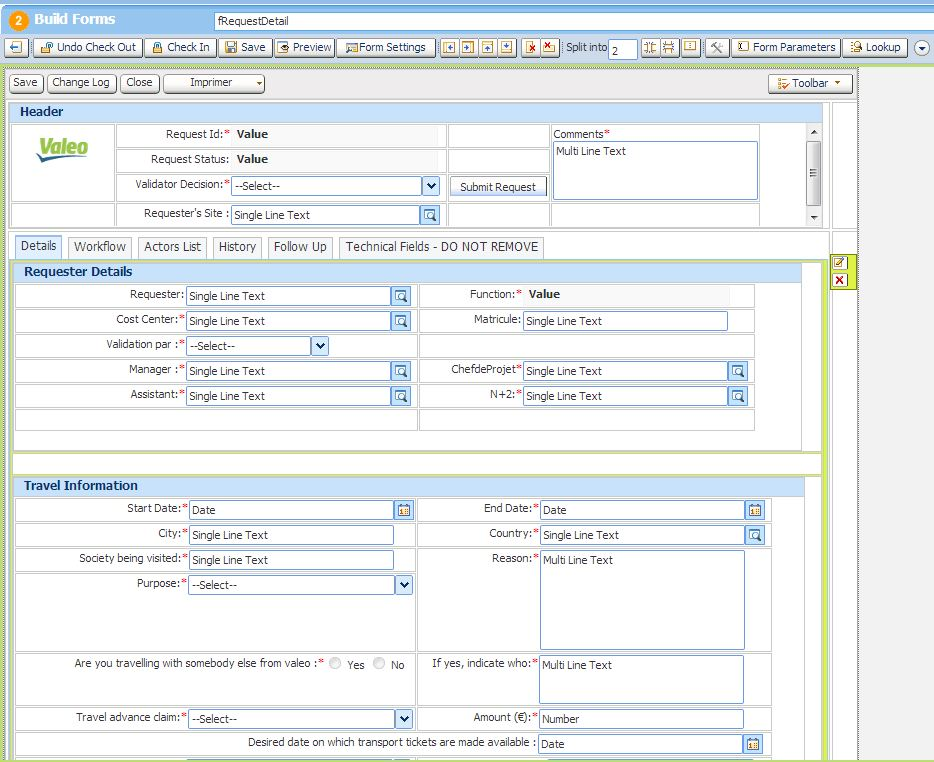
\includegraphics[height=14.5cm]{cordysDevFormsDef.jpg}
	\caption{\textit{Interface de développement de Cordys - Interface de définition des Formulaires}}\label{image.cordysDevFormsDef} 
\end{figure}

\clearpage
\subsubsection{L'onglet ``Business Process"}

C'est la notion clé du système Cordys, et d'ailleurs mon sujet de stage mentionne cet élément sous le nom de \textbf{Workflow}. Ce n'est donc pas un outil à proprement parlé mais plutôt une finalité: sa mise en place.

Un Business Process est donc un ensemble d'activités liées qui produisent un service de manière à atteindre les objectif du business. Les ``Business Processes" sont \textbf{la manière} d'effectuer une tâche spécifique au sein d'une organisation spécifique. 
Un Business Process définit, dans notre cas, un parcours de validation ou signature et ainsi aide les employés à interagir avec les différentes entités de l'entreprise.



Pour exemple, prenons l'approbation du remboursement d'une note de frais :

Un employé peut avoir des dépenses durant un voyage d'affaire et doit être remboursé. Ainsi il serait intéressant d'établir un \textbf{Business Process} décrivant le parcours de signature à effectuer de manière à donner l'autorisation de manière automatique à la finance pour le paiement de la note de frais:\\
Demande de remboursement => Validation du supérieur hiérarchique => Validation du chef de projet => Demande de remboursement validée. \\
Il peut être judicieux de notifier tout le monde dès l'acceptation ou le refus de la demande. Le remboursement peut ainsi être débloqué par le service financier.

Automatiser ce genre de processus permet d'une part de limiter les erreurs humaines et d'autres part d'en maximiser l'efficience et la traçabilité.

Un Business Process se définit par:

\begin{itemize}\itemsep7pt

	\item \textbf{Un But: } Un Business Process possède un but bien défini, qui est le besoin Business d'une action systématique.
	
	\item \textbf{Des données en ``entrée": }Un Business Process a besoin de données en entrée, que l'on appelle ``ressources", pour fonctionnner. Pour exemple, reprenons notre exemple de la validation des notes de frais. Voici quelques ressources : Date du début du Voyage, Date de fin du voyage, montant de la note de frais, Utilisateur demandeur ...
	
	\item \textbf{Des données en ``sortie: "}Un Business Process produit une ou plusieurs sorties qui fournissent des informations importantes pour l'entreprise.
	
\end{itemize}

Il est possible de publier un Business Process et de l'intégrer à un formulaire à la manière d'un Web Service. Il est ensuite possible de définir les ``déclencheurs" qui vont appelés le Business Process à intervalle régulier ou sous certaines conditions.

\begin{figure}[H]
    \centering
    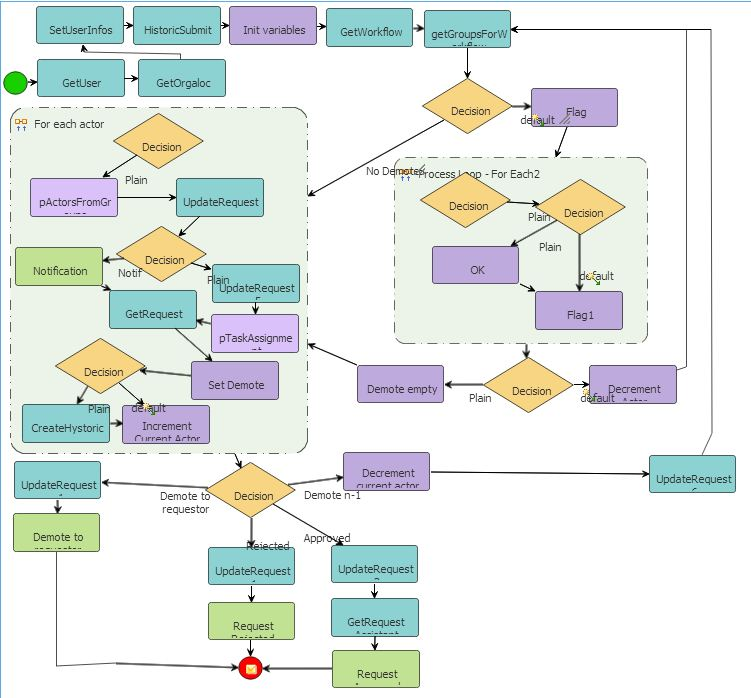
\includegraphics[height=17cm]{cordysDevBusinessProcess.jpg}
	\caption{\textit{Interface de développement de Cordys - Exemple d'un Business Process}}\label{image.cordysDevFormsDef} 
\end{figure}

\clearpage

\subsubsection{L'onglet ``Business Rules"}

Les ``Règles Business" sont des collections de procédures qui commandent une organisation et les services qui lui sont rattachés. Ils définissent les contraintes qui s'appliquent et aident à suggérer les activités clés du Business Process au moment opportun. Ils préparent et présentent les données de manière à faciliter les prises de décision critiques et stratégiques. 

Une ``règle Business" peut appeller un Business Process, envoyer des notifications, ou afficher des avertissements. Par exemple, une règle Business peut orienter le choix d'un Business Process ou d'un autre en fonction du montant de la note de frais pour reprendre notre exemple. (Si le montant de la note de frais est supérieur à 1000€ => Demander la validation du Directeur d'usine). 

Pour résumer, une règle Business est un ensemble de conditions et d'actions. Structure algorithmique classique en \emph{IF-THEN } et multiples \emph{ELSE-IF}.


Voici le type d'actions que peut effectuer une ``règle Business" lorsqu'une de ses conditions d'exécution est vérifiée:

\begin{itemize}\itemsep7pt
	 \item \textbf{Assigner une valeur à un champs d'un formulaire ou d'un Application Object.}
	 	 
	 \item \textbf{Arrêter une transaction en cours et en notifier l'utilisateur par l'affichage d'un message.}
	 
	 \item \textbf{Envoyer une notification à un utilisateur.}
	 
	 \item \textbf{Déclencher un Business Process.} 
\end{itemize}

\subsubsection{L'onglet ``Web Services"}

Un Web Service  est une fonction logicielle construite pour réaliser des interactions machine à machine par l'intermédiaire d'un réseau. Ils utilisent un modèle standardisé de données comme: XML / SOAP / WSDL. XML est utilisé pour le formatage des données, SOAP pour effectuer le transfert des données, et WSDL pour décrire le service.

Les Web Services permettent une communication entre plusieurs applications originaires de différentes sources, le tout avec un temps de réponse au plus court et une compatibilité multi-plateforme grâce au formatage XML des données.\\
Ainsi une application en Java peut communiquer avec une application en Perl fonctionnant sur Unix ou Windows.

Cordys permet une génération automatique d'une série de Web Services Standards pour chaque Application Object : Lecture, Ecriture, Modification, Suppression.\\
Il est également possible de construire des Web Services plus avancés grâce à l'assistant dédié.

\clearpage

\subsubsection{L'onglet ``Configure Application"}

Après la création et le paramétrage de tous les éléments de l'application, il devient nécessaire de configurer l'application et ses différents onglets.

Ces onglets peuvent regrouper un ou plusieurs formulaires et chaque formulaire et/ou onglet peut être accessible ou non en fonction du privilège utilisateur.

Les privilèges utilisateurs sont à créer et à modifier dans cette section. Seul le droit administrateur est automatiquement en place, il permet un accès total à l'application.

Il est également possible de référencer une application comme source, cette dernière sera accessible à travers l'application actuelle (en particulier lors des Look-Ups)

\subsubsection{Creation d'un ``\emph{Application Package}"}

Une fois l'application prête pour être testée dans le mandant de test, il est nécessaire de générer un "Application Package" soit dans le but de créer une sauvegarde de l'application à l'instant T soit pour la déployer dans un autre mandant.
\clearpage

\section{Titre de Fonction : ``Automation Analyst"}

\subsection{Description de mon rôle}

Mon rôle a été principalement orienté sur deux objectifs. En effet il m'a été demandé d'une part, de développer des améliorations sur un parc applicatif existant (en particulier par rapport aux attentes des ``Business Owners") ainsi que de développer et de déployer de nouvelles applications, d'autres part, il m'a été demandé d'effectuer le support applicatif sur ces mêmes applications via un système open source de tickets: GLPI.\\
Finalement, il m'a été demandé d'effectuer des formations \emph{orientées utilisateur} sur plusieurs sites Français à propos de l'utilisation des applications déployées en production.

Ce genre de poste demande donc une double compétence:

\begin{itemize}\itemsep7pt

	\item En effet, il nécessaire de connaître parfaitement son outil et la plateforme afin de développer la fonction qui manque ou d'améliorer l'interface d'une application. Une faculté d'analyse et d'adaptation rapide sont donc les qualités humaines prépondérantes dans cette activité en plus des connaissances techniques.
	
	\item Le deuxième rôle est d'effectuer un support relatif à une quinzaine d'applications. Il est donc extrêmement courant de d'interagir avec tout type d'utilisateur et ce plusieurs fois par jour. Le problème réside dans le fait que l'on ne connait que rarement son interlocuteur, tout comme sa fonction dans l'entreprise. Il faut donc être capable d'adapter son discours en fonction des connaissances de l'utilisateur, de son ``empressement" et de sa fonction dans l'entreprise. Il est donc critique d'avoir de bonnes facultés de communication (en anglais et français), une certaine capacité de discernement et de répartie.
	
\end{itemize} 

\clearpage

\subsection{Retour sur expérience}

\subsubsection{La partie technique}

Concernant la partie technique, Cordys Process Factory est très peu documenté. Impossible de trouver un manuel ou même une documentation officielle. Valeo possède ses propres modules de formation mais cela reste très succinct et ce fût très complexe de me former à  son utilisation, l'administration de la plateforme et particulièrement au développement sur cette plateforme. Malgré une formation intensive de deux jours à Paris, autonomie et des dizaines d'heures à tâtonner sur la plateforme furent les maitres mots de mon expérience sur Cordys Process Factory.

Un Forum Valeo pour les développeurs sur Cordys est en place, cet outil me fut d'un grand secours, surtout durant les premiers mois de mon stage.
Malgré cela je ne pense toujours pas maitriser la plateforme. Je connais les fonctions et les éléments qui me permettent de faire ce dont j'ai besoin, mais sur une demande trop spécifique ou trop pointue il m'est nécessaire de demander de l'aide. Cordys est une plateforme propriétaire de \textbf{développement au clic}, très peu de code est à mettre en place. Ce qui signifie que si vous ne savez pas où cliquer pour effectuer telle ou telle action, vous pouvez chercher pendant des heures avant que la solution vous apparaisse. A l'inverse d'un langage de programmation qui, pour la plupart, malgré ses spécificités, reste similaire à de nombreux autres et avec de solides connaissances en algorithmique et une documentation il est relativement aisé d'arriver à ses fins.

\subsubsection{La partie communicationnelle}

C'est sans aucun doute la partie qui m'a demandé le plus d'efforts. Tant dans la forme que dans le fond. En effet, je m'étais majoritairement adressé, auparavant, à des personnes connaissant l'informatique dans le cadre de mes études. Et ce ne fut pas forcément aisé d'adapter mon discours aux connaissances de mon interlocuteur et surtout au fait que je ne sache jamais à qui je m'adresse. Un environnement comme celui de Valeo est très complexe et demande de grandes précautions lorsque l'on s'adresse à quelqu'un. Il est donc primordial d'\textbf{apprendre} à ne s'engager sur quelque chose même si on le croit acquis et 100\% sûr. En effet, ce qui est possible dans un environnement quelconque n'est pas forcément possible dans l'environnement Valeo. A la fois d'un point de vue technique et également parce que l'on ne maitrise pas tous leviers d'une action et qu'il faut obtenir l'accord d'un certains nombre de personnes avant de pouvoir déclencher certaines actions.

J'ai personnellement eu beaucoup de mal à gérer la pression durant les deux premiers mois. En effet, un environnement comme Valeo demande que tout soit fait en flux tendu et en parallèle voir limite ``pour hier" pour ne paraphraser personne. C'est une situation à laquelle je n'avais jamais fait face, il a fallu \textbf{apprendre} à ne pas paniquer et se recentrer sur l'objectif, définir des priorités, gérer les timings et le tout de manière relativement automatique et intuitive car il n'est pas envisageable de passer plusieurs heures par semaine à établir un diagramme de Gantt pour la semaine. La \emph{liste des tâches} à effectuer de Google fut sans aucun doute mon meilleur allié pendant ce stage.

\clearpage

\chapter{Un Système ERP : SAP}
\section{Un système ERP : SAP}

%http://dspace.bracu.ac.bd/bitstream/handle/10361/1559/U2K2%20Project%20and%20SAP%20Execution.pdf?sequence=1
%

\subsection{SAP, vue d'ensemble}

SAP est un ERP (\emph{Enterprise Resource Planning} ou en français :  \textbf{Planification des Ressources de l'Entreprise}) développé par la société éponyme. Ce sigle signifie :\textbf{Systems, Applications, and Products for data processing}.

SAP est un puissant outil qui intègre de multiples Business Process et Fonctions en un seul système unifié. Fonctionnant sur une architecture Client / Serveur classique, chaque utilisateur (disposant des droits nécessaire) peut facilement gérer et tracer les ventes, la production, les finances de l'entreprise et les ressources humaines en temps réel. 

SAP est un système modulaire qui se compose de plusieurs parties. Chacune de ces parties peut elle même se diviser en plusieurs sous modules de fonction spécifique.
Tous les modules SAP sont cependant inter-connectés via une base de données centralisée qui connecte et recoupe les différents aspects et les différentes données de l'entreprise.

Pour n'en citer que quelques exemples, voici les quelques modules utilisés chez Valeo:

\begin{itemize}
	\item \textbf{Module MM: }``Material Management" est le module logistique de SAP. Il gère les stocks, et les mouvements de stocks : entrées, sorties, et transferts.
	
	\item \textbf{Module PP: }``Production Planning" concerne la planification de la Production.
	
	 \item \textbf{Module SD: }``Sales and Distribution concerne l'administration des ventes.
	 
	 \item \textbf{Module FI: }``Financial contient toutes les écritures des ventes et achats, lesquelles se déversent dans la comptabilité générale via la comptabilité client ou fournisseur.
	 
	 \item \textbf{Module CO: }``Controlling concerne le contrôle de gestion.
	 
	 \item \textbf{Module BW: }``Business Information Warehouse est un outil de fouille de données et par extension de Reporting.
	 
\end{itemize} 

\clearpage

\subsection{Les intérêts Business de l'utilisation du système SAP}

De nombreuses entreprises utilisent de nos jours des systèmes d'information qui ont été mis en place pour exécuter un certains nombre de tâches spécifiques tout en apportant un outils de d'analyse et d'extraction des données transitant au sein du système.\\
Certains sont même capable de fournir des données temps-réels de l'état du système. En effet ces systèmes possèdent toutes les informations nécessaires en leur sein pour permettre une utilisation rapide et multi-support afin de gérer tout type d'évènements. 

Typiquement, une compagnie possédant de nombreux systèmes sous son contrôle, et différents processus critiques à gérer en parallèle comme la production, la vente, la comptabilité, ... aura un système d'information d'un grande complexité.  Chacun de ces systèmes fonctionnant avec une base de données bien spécifique. \\
Des interfaces de transfert de données entre ces systèmes sont utilisés aussi souvent que nécessaire. Le système devient très rapidement complexe et difficile à gérer. Le plantage d'un des éléments de tout le système d'information impliquera un service dégradé sur la globalité du système. Les coûts de maintenance, de sauvegarde ainsi que de maintient d'un DRP efficace deviennent prohibitifs.

SAP propose une vision différente, une vision unifiée: Un seul système d'information dans le système : SAP. 

Toutes les applications peuvent accéder aux données communes du système. Chaque événement qui a lieu dans le système est enregistré dans le système et immédiatement accessible par l'ensemble des modules. L'utilisation d'un système ERP permet une amélioration de la cohérence des données et de l'efficience du système. La simplification des actions, transactions et des processus réduit de plus la charge sur le système global. 

\clearpage
\section{Le projet Comp@ssV4}

\subsection*{Préambule}

J'ai travaillé uniquement sur la partie qui concerne la migration et la nettoyage des données des clients dans le système SAP.
Le système SAP étant trop vaste, il m'est impossible de m'étendre sur tous les sujets. Je n'expliquerai donc dans ce rapport que les interactions à ce sujet.

Ce projet porte le nom de Comp@ssV4: \emph{Corporate Operationnal \& Management Performance @dvanced SyStem}.
Il succèdera à Comp@ssV2 et non à Comp@ssV3 qui fut un projet avorté et non poursuivi suite à un changement de politique interne.

\subsection{Une migration logicielle et architecturale}

Cette migration porte sur deux aspects :

\begin{itemize}
	\item Une mise à jour du logiciel.
	\item Un changement de l'architecture serveur (au regard des clients) pour une version plus unifiée.
\end{itemize}

\subsubsection{Mise à jour du logiciel}

Comme tout logiciel, il est maintenu pendant un certains temps. La version actuelle n'étant plus maintenue, il est nécessaire dans un environnement comme celui de Valeo de mettre à jour son système afin de réduire ses coûts de maintenance.

\subsubsection{Changement de l'architecture serveur}

En plus de la mise à niveau du logiciel SAP, Valeo a décidé de revoir entièrement son architecture applicative SAP et plus spécialement celle des clients.
Une vision plus unifiée et plus centralisée a été pensée et mise en place afin de correspondre aux exigences de la nouvelle politique du Groupe Valeo.
\clearpage

\subsubsection{Ancienne Structure: Comp@ssV2}

L'architecture de Comp@ssV2 peut être décrite comme ceci : 

 \begin{figure}[H]
    \centering
    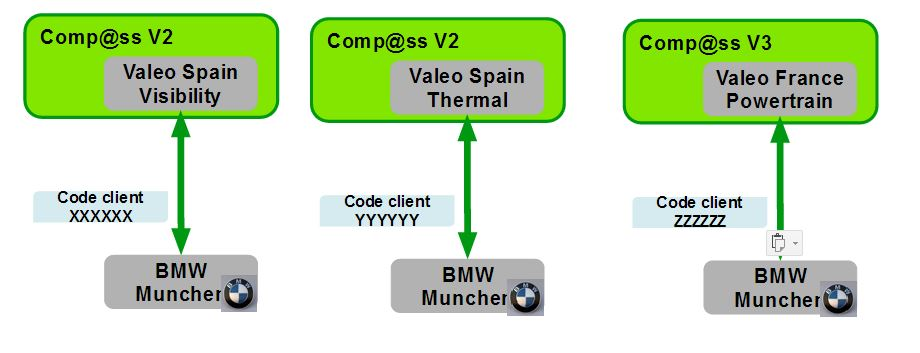
\includegraphics[height=7cm]{compassV2Customer.jpg}
	\caption{Structure du système Comp@ssV2 - Pas de référentiel client}\label{image.compassV2Customer} 
\end{figure}

\subsubsection{Nouvelle Structure: Comp@ssV4}

L'architecture de Comp@ssV4 peut être décrite comme ceci : 

 \begin{figure}[H]
    \centering
    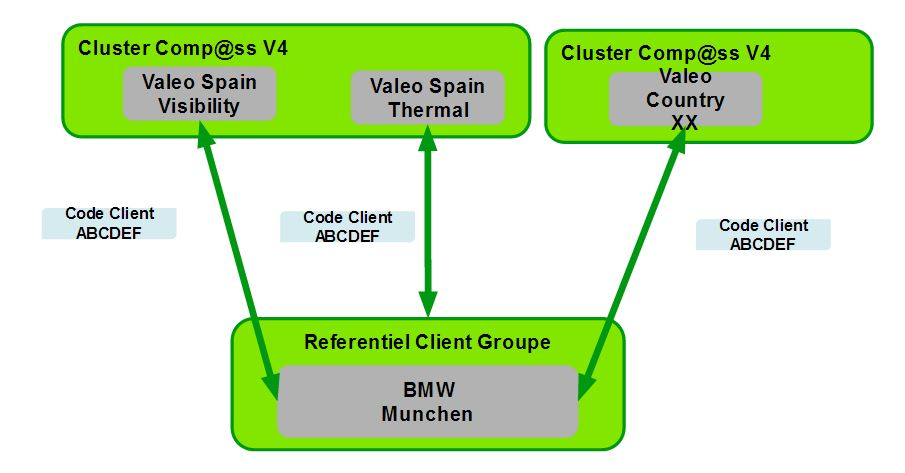
\includegraphics[height=9cm]{compassV4Customer.jpg}
	\caption{Structure du système Comp@ssV4 - Présence d'un référentiel client Groupe}\label{image.compassV4Customer} 
\end{figure}

\clearpage

\subsubsection{Résumé de la migration}

Ainsi, c'est une migration biaxiale qui est en cours de réalisation.\\
Cependant, la partie logicielle n'étant pas de notre périmètre, je ne m'étendrai pas sur ce sujet.

Ainsi, pour résumer, il est établi que toutes les machines SAP de Valeo pointeront vers un annuaire SAP de clients.\\ Ainsi chaque site aura une codification unifiée et cohérente avec les autres.
Le client numéro 1 sera le même quelque soit le système SAP de Valeo.

 \begin{figure}[H]
    \centering
    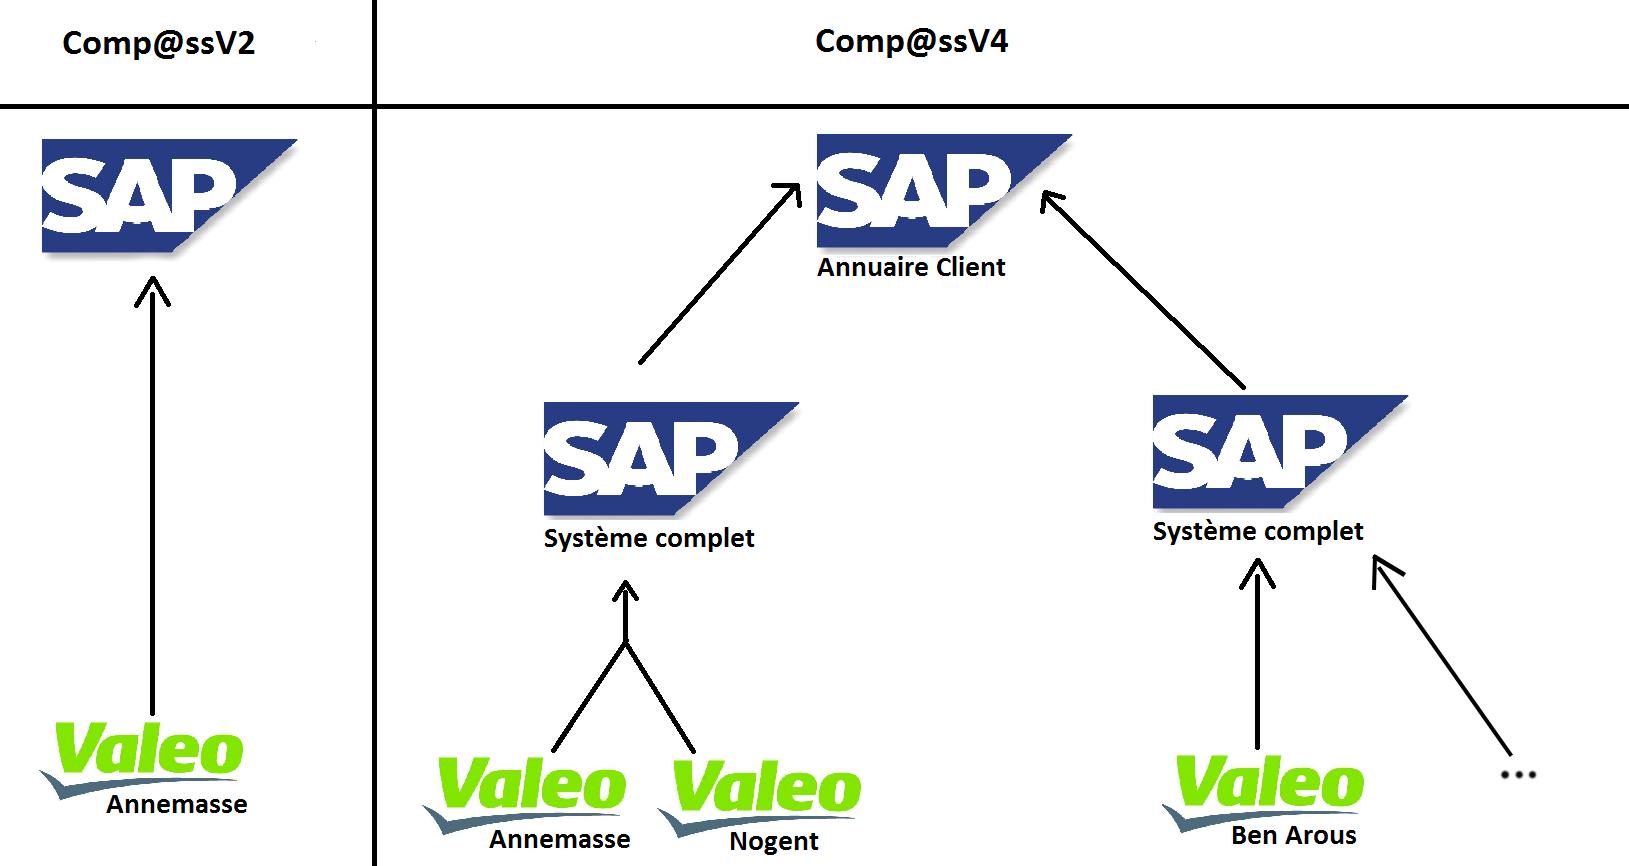
\includegraphics[height=10cm]{compassNewOrga.png}
	\caption{Comp@ssV2 vs Comp@ssV4 - Nouvelle Architecture Client}\label{image.compassNewOrga} 
\end{figure}
\textbf{
Les avantages d'une telle structure sont:}

\begin{itemize}\itemsep7pt
	\item Avoir une codification commune à tout le groupe Valeo. 
	\item Faciliter la comparaison entre les prévisions et les ventes réelles. 
	\item Faciliter la communication entre les sites Valeo. 
	\item Avoir une autorité commune sur un annuaire client unifié.
	\item Être capable de consolider le changement et les modifications des clients au niveau mondial.
	\item Avoir une vue globale du Business réalisé avec un client.
\end{itemize}

\clearpage
\section{Un client = Une fonction partenaire}

\subsection{Les différentes fonctions partenaires}

Un client peut, classiquement, être référencé sous quatre formes dans un environnement professionnel.

\textbf{Ainsi nous y retrouvons:}

\begin{itemize}\itemsep7pt
	\item Le client \textbf{Donneur d'ordre}, fonction partenaire AG dans SAP (de l'Allemand: \textit{\textbf{A}uftrag\textbf{g}eber})
	\item Le client \textbf{Livré}, fonction partenaire WE dans SAP (de l'Allemand: \textit{\textbf{W}aren\textbf{e}mpfänger})
	\item Le client \textbf{Facturé}, fonction partenaire RE dans SAP (de l'Allemand: \textit{\textbf{R}echnungs\textbf{e}mpfänger})
	\item Le client \textbf{Payeur}, fonction partenaire RG dans SAP (de l'Allemand: \textit{\textbf{R}e\textbf{g}ulierer})
\end{itemize}

\subsubsection{Un exemple simple sur les fonctions partenaires}
Prenons une situation simple et courante pour expliquer que sont ces fonctions partenaires.

\textbf{Un enfant} veut acheter un cadeau à sa maman pour la fête des mères, pour cela il se connecte sur son site en ligne préféré et choisi ce qu'il veut commander.\\
Il passe la commande, seulement étant enfant il n'a pas de carte bancaire et ne peux donc payer ... \textbf{Papa} aide donc son fils à passer commande avec sa carte bancaire.\\
Une semaine plus tard, \textbf{Maman} reçoit le colis.

Dans cette histoire, l'\textbf{enfant} fait office de donneur d'ordre: C'est lui qui effectue la commande. \textbf{Papa} quand à lui grâce a sa carte bancaire est devenu le client payeur et le client facturé. Quand à \textbf{Maman}, elle est donc le client livré. 

Pour résumer:

\begin{itemize}\itemsep7pt
	\item Enfant = Client Donneur D'ordre = \textbf{AG}
	\item Papa = Client payeur et Client Facturé = \textbf{RE \& RG}
	\item Maman = Client Livré = \textbf{WE}
\end{itemize}
	
Cette explication est primordiale pour la suite car dans un contexte industriel il est très courant d'avoir quatre clients différents pour chacune des fonctions partenaires pour une seule et même commande.
	
Il est donc \textbf{nécessaire} d'établir une codification uniforme pour chacune de ces fonctions partenaires.

\clearpage


\section{Reprise des clients dans Comp@ssV4}

\subsection{Deux groupes de clients: ``Cluster" et ``Référentiel Groupe"}

Dans le contexte du projet Comp@ssV4, tous les clients ne seront pas repris au niveau du référentiel commun groupe.\\
Les autres seront définis uniquement au niveau de l'instance "Cluster", c'est à dire le système SAP sur lequel fonctionne le site Valeo car ces clients lui sont propres et ne sont pas partagés avec les autres sites.
\begin{figure}[H]
    \centering
    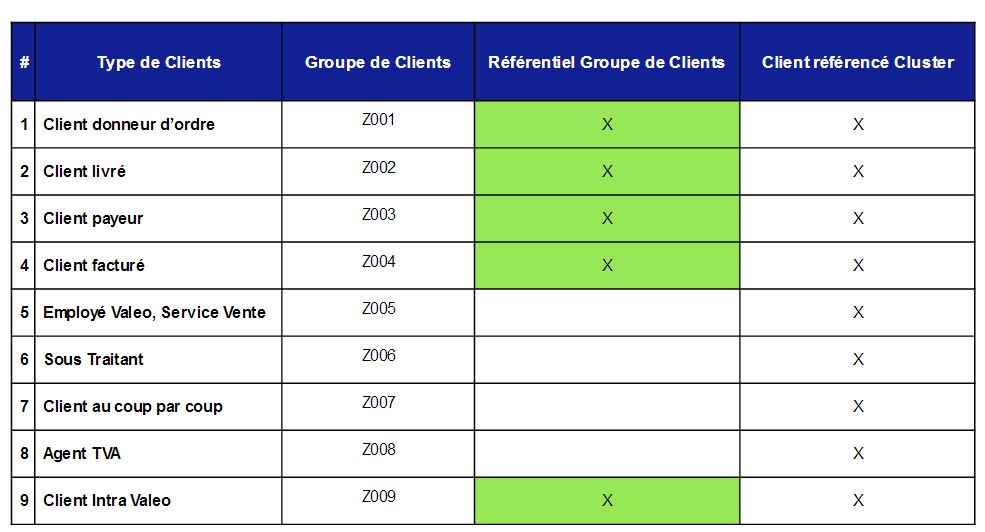
\includegraphics[height=6.5cm]{compassCustomerGroup.jpg}
	\caption{Reprise des clients Comp@ssV2 - Referentiel Groupe vs Cluster}\label{image.compassCustomerGroup} 
\end{figure}

\subsection{Cadre de reprise d'un client}
Il n'est pas cohérent de reprendre tous les clients des systèmes SAP de tout Valeo. En effet, certains ne sont plus actifs, n'existent plus, ont déménagés, ou n'ont tout simplement plus aucune activité avec Valeo.

Ainsi chaque site Valeo, devra choisir parmi ses clients comp@ssV2, ceux qui répondent à l'ensemble des critères suivant:

\begin{itemize}\itemsep4pt
	\item Tous les clients non marqués ``à supprimer" (On ne supprime jamais rien, on applique des marqueurs de suppression dans un système ERP: soucis de traçabilité).
	\item Tous les clients ayant effectué une commande durant les 2 dernières années.
	\item Tous les clients avec une commande non clôturée (en cours ou en litige ou en attente de paiement)
\end{itemize}

Tous ces filtres sont ajoutés à l'outil d'extraction que nous utilisons: \href{http://www.informatica.com/us/SAP/}{\textbf{Informatica}}.


\clearpage

\section{Une nouvelle codification client}

\subsection{Presentation de la nouvelle codification}

\begin{figure}[H]
    \centering
    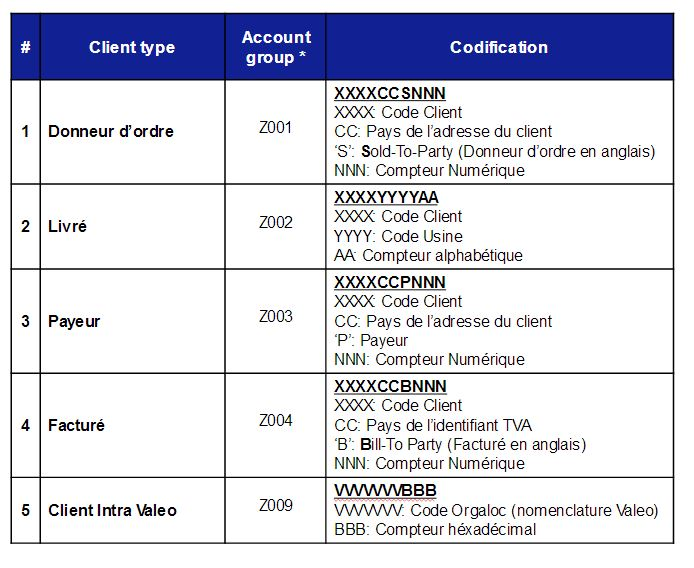
\includegraphics[height=11cm]{compassCustomerCodification.jpg}
	\caption{Nouvelle Codification Client du système Comp@ssV4 - Codification Unifiée}\label{image.compassCustomerCodification} 
\end{figure}

La codification Comp@ssV4 assure que chaque client ne correspondra qu'à\textbf{ une seule fonction partenaire} et non plusieurs comme cela était parfois le cas dans Comp@ssV2. Ainsi un client du groupe Z001 n'aura qu'une fonction partenaire : AG au lieu de AG/WE/RE et RG, comme parfois, dans Comp@ssV2.

La codification Comp@ssV4 définit le \textbf{code Client étant unique}. Ainsi deux clients différents auront un code client différent (exemple: \textit{Renault et BMW}), par contre deux clients du même Groupe (au sens entreprise) auront un code client commun (exemple: Renault Douai et Renault Compiegne).

La codification Comp@ssV4 définie le code usine de manière unique quelque soit l'entreprise et l'usine. Ainsi deux usines ne peuvent avoir en aucun cas le même numéro (Exemple: Renault Douai, Renault Compiegne et BMW Munich auront tous les trois un code Usine obligatoirement différent).

\section{Processus de migration de Comp@ssV2 à Comp@ssV4}

\begin{figure}[H]
    \centering
    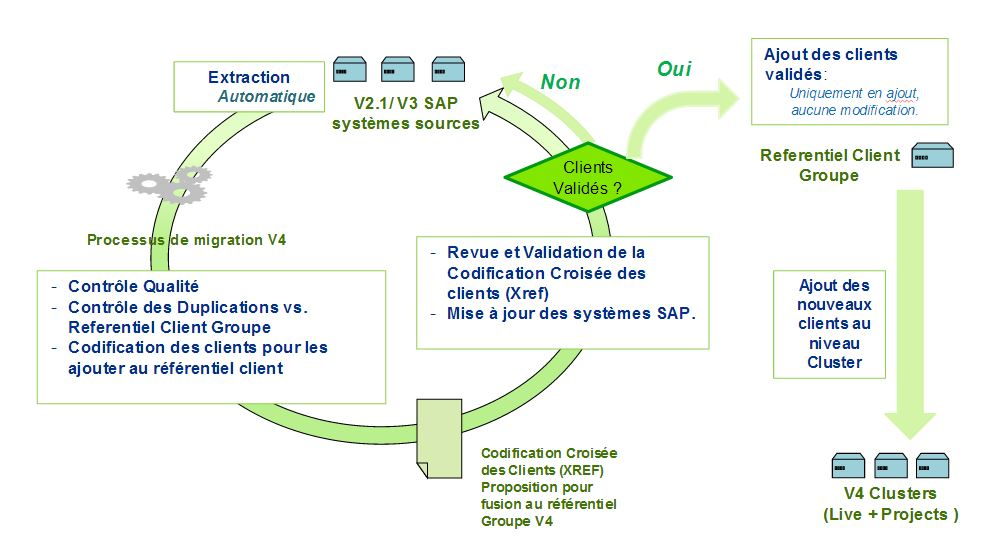
\includegraphics[height=12.5cm, angle =90]{compassV4MigrationProcess.jpg}
	\caption{Processus de migration de Comp@ssV2 à Comp@ssV4}\label{image.compassV4MigrationProcess} 
\end{figure}



\section{Explication du travail effectué}

\subsection{Définition de l'objectif}

Afin de mener à bien la migration de Comp@ssV2 à Comp@ssV4, il nous a donc été demandé de réaliser le nettoyage des données Clients et d'en effectuer la reprise pour Comp@ssV4.

La reprise consiste à faire correspondre autant que possible les clients déjà codifiés par les autres sites dans le référentiel Client Groupe de Comp@ssV4. Pour les autres, nous serons tenus de les codifier en respectant les règles de codification afin de les intégrer dans le système.

La problématique qui s'est donc posée à nous est la suivante:

\textbf{``Comment réaliser une comparaison efficace entre les clients Comp@ssV2 de notre système et ceux du référentiel groupe déjà codifiés dans le nouveau système ?"}

Effectivement, il est difficilement pensable de recouper et de comparer plus de 2500 clients de notre système avec les 6000 clients déjà existant dans le référentiel à la main.\\
Il nous a donc fallu trouver un outil pour effectuer cette comparaison.

\clearpage

\subsection{L'algorithme de Ratcliff et Obershelp}

Grâce à un cours sur la détection de la redondance des données que j'avais suivi en Erasmus à Vienne, j'ai pu proposer l'algorithme mis au point par \textbf{Ratcliff et Obershelp} sur la détection de séquence dans les chaines de caractères.

Cet algorithme renvoie \textbf{un pourcentage de ressemblance} entre deux chaines de caractères qu'il reçoit en entrée.

Cet algorithme permet de répondre à notre besoin pour les raisons suivantes:


\begin{itemize}\itemsep7pt
	\item Possibilité ``d'absorber" de faibles variations: Chaque site Valeo n'a pas forcément identifié l'adresse ou le nom complet du client de la même manière. Il est donc nécessaire d'établir une \textbf{marge d'erreur} lors de la reconnaissance automatique.
	\item Algorithme de relativement faible compléxité: $N^2$.
\end{itemize}

\subsubsection{Principe de l'algorithme}

L'algorithme de Ratcliff et Obershelp calcule la similarité entre deux chaines de caractères de la manière suivante:\\

\textbf{2 * (nombre de caractères identiques) / (nombre de caractères dans les deux chaines)}

Correspondance des caractères dans un premier temps de manière relative à leur position (\textit{le caractère 1 de la chaine 1 correspond-il au caractère 1 de la chaine 2 ?}), le tout sur la plus longue sous-séquence en commun (les chaines n'ont pas forcément la même taille). A cela s'ajoute de manière récursive la correspondance des caractères non associés toujours en cherchant la plus grande zone correspondante et le tout jusqu'à ce que plus aucune association ne soit possible.

\textbf{Exemple:}

La similarité entre ALE\textbf{X}ANDRE et ALE\textbf{KS}ANDER est égale à:


\begin{tabular}{|>{\centering\arraybackslash}p{18cm}|}
  \hline
  ~\\
  \textbf{2 * (3+3+1+1) / (9+10) = 0.84}  (Corresponds : \textbf{ALE} (3), \textbf{AND} (3), \textbf{E}(1), \textbf{R}(1))\\
  ~\\
  \hline
\end{tabular}

\clearpage

\subsection{Objectifs de notre méthode}

L'objectif est d'être capable de \textbf{détecter} une forte similarité entre deux clients. Mais il ne nous semblait pas judicieux de réaliser l'association de manière \textbf{automatique} pour des raisons de contrôle des données (l'impact d'une erreur est important car cela touche les clients de Valeo).

Deux objectifs apparaissent donc:

\subsubsection{Limiter les ``faux positifs"}

Afin d'effectuer notre travail de manière efficace il est important d'effectuer un \textbf{tri}, entre les clients qui ne correspondent \textbf{pas}, ceux qui correspondent \textbf{un peu}, et ceux qui correspondent \textbf{beaucoup}.

Par souci de temps, nous avons choisi de nous focaliser sur ceux qui ont un fort taux de ressemblance (avec la méthode précédemment expliquée).

Il parait donc essentiel de limiter ce que nous appellerons un \textbf{faux positif}:
Un faux positif c'est deux clients qui semblent identiques mais qui en réalité ne le sont pas (Exemple: Renault Toulouse et Renault Toulon).

Nous devons donc définir un \textbf{seuil} de détection de manière à ne pas générer trop de pollution dans nos résultats.

\subsubsection{Aucun ``faux négatif" ou presque}

Encore plus gênant qu'un faux positif, nous avons le faux négatif. Cette fois ci nous avons deux clients identiques et malheureusement identifiés de manière trop différentes et le taux de ressemblance est en dessous de notre seuil de détection. Conséquence: Nous perdons une association et ce client sera donc recodifié, ce qui va à l'encontre du principe même du projet (limiter le nombre de client et une codification unique pour un même client au sein de tout Valeo).

\subsection{La problématique du seuil de détection}

Nous avons effectué de nombreux tests afin de déterminer quel était le \textbf{meilleur} seuil de détection afin de ne pas générer trop de pollution (faux positifs) et surtout de ne rater aucune correspondance ou presque (faux négatifs).

\textbf{Suite aux tests effectués nous en avons déterminer le seuil de : 60\%}

\subsection{Principe de l'outil que nous avons développé}

Afin de répondre au besoin, nous avons donc établi un outil permettant de recouper les clients V2 avec les clients V4.

Cet outil cherche à réaliser des paquets de clients V2 et V4 ayant une forte ressemblance. Ces paquets sont constitués dans un fichier excel tierce qui pourra être utilisé comme fichier de travail. Le fichier des clients extrait reste inchangé pour des raisons de corruption de données en cas d'erreur de manipulation.

Cet outil a été développé par mes soins en VBA et implémenté sous forme de macro \textbf{instable} dans Excel par le biais du fichier spécialisé excel : \textbf{*.xla}.

\textbf{Voici un bref descriptif de son fonctionnement :}

\begin{enumerate}
	\item Génération de la clé de comparaison par concaténation des champs \textbf{importants} dans notre analyse : \textit{nom, ville, adresse}
	\item Réalisation d'une boucle x $\in$ V4 qui analyse la ressemblance entre y $\in$ V2 et x. 
	\item Si ressemblance (x,y) > 60 \% $\rightarrow$ Constitution d'un paquet dans le fichier excel de sortie.
	\item A chaque fois que l'outil trouve une ressemblance entre V2 et V4, il procède également à l'analyse de V4 par rapport à V4. Cela permet de balayer dans les deux sens la liste des clients et de constituer des paquet plus cohérent et non des associations 1:1.
\end{enumerate}

\subsection{Les principales difficultés que j'ai rencontrées}

Je ne connaissais pas le VBA et ce ne fut pas forcément aisé d'obtenir le résultat escompté immédiatement voir même de \textit{débugguer} ...

De plus la structure de l'algorithme n'étant pas simple, j'ai dû passer beaucoup de temps en phase de conception afin d'obtenir le schéma le plus efficace et fonctionnel possible.

Le langage VBA, celui des macros excel, n'est pas forcément très rapide. Les accès mémoire et encore plus les écritures ne se font pas rapidement. Ainsi après réalisation de la macro j'ai procédé à une longue phase de recherche et d'optimisation sur la rapidité des différentes fonctions pour effectuer certaines tâches. J'ai divisé le temps d'éxécution par un facteur 3. Et malgré tout l'exécution a tout de même durée près de deux heures et demi.

\clearpage

\subsection{Quel futur pour cet outil}
A ma grande surprise, l'outil mis en place intéresserait les responsables du projet au niveau Groupe. Il m'a été demandé de leur faire une présentation de l'outil à la fois dans le principe et dans l'utilisation.

Il m'a été demandé en ce sens de le modifier afin qu'il soit \textbf{industrialisable} et  \textbf{utilisable par un non informaticien}: comprendre sans modification du code.

Cette nouvelle a récompensé les efforts que l'équipe a pu mettre dans le projet et permet de mettre un point final, pour ma part, sur ce projet au regard de l'échéance de mon stage.
\clearpage

\chapter{Conclusion}

C'est avec plaisir que, maintenant, je peux regarder en arrière, rire de mes erreurs, sourire de mes nombreuses questions mais surtout être satisfait du chemin parcouru.

Les nombreux problèmes qui se sont posés à moi m'ont forcé à toujours aller plus loin dans mes raisonnements et mes recherches, à trouver \textit{la parade} ou \textit{l'astuce} qui fera que \textit{cette fois-ci, ça marchera}.

Ce fut également un moment où j'ai pu tiré profit de l'enseignement reçu à l'UTC ainsi que lors de mes deux Erasmus à Vienne et Hamburg. Ce fut également l'occasion de mettre en difficulté mes connaissances afin de consolider mes acquis.

J'ai eu l'occasion d'acquérir une première expérience du monde de la recherche avec un projet concret : METIS. Mais également l'opportunité de découvrir un cas concret d'utilisation de la Vision par Ordinateur et de l'apprentissage automatique. Ce fut également une chance unique de découvrir le monde du développement logiciel et le développement de services basés sur le cloud mais également d'entrevoir les problématiques et challenges de la rétro-conception de grands ensembles mécaniques.

J'en profite, encore une fois, pour remercier tout ceux qui ont participé au bon déroulement de ce stage. 

Je ne saurais faire la liste de tout ce que j'ai pu apprendre, cette expérience me sera très utile pour la suite de mon projet professionnel: Réaliser une thèse sous la direction de M. Durupt à l'UTC et la codirection de M. Kiritsis à l'EPFL. Il est un premier élan dans le monde de la recherche et un point final à mon cursus d'ingénieur.

% Pour finir l'interligne de 1,5
%\end{onehalfspace}

%----------------------------------------
% Pour la bibliographie
%----------------------------------------
% Citer tous les ouvrages/références
\nocite{*}

\bibliography{IEEEabrv,biblio}

\printindex

\appendix

\pagebreak

\chapter*{Rédaction du Rapport en langage LaTeX}
\markboth{Langage LaTeX}{}
\addcontentsline{toc}{chapter}{Rédaction du Rapport en langage LaTeX}
Ce rapport a été entièrement rédigé en \href{http://fr.wikipedia.org/wiki/LaTeX}{\textbf{LaTeX}}. 

Les sources sont disponibles et téléchargeables sur Github à l'adresse suivante :\\
\href{https://github.com/JonathanDekhtiar/Rapport-TN09}{\textbf{https://github.com/JonathanDekhtiar/Rapport-TN09}}. 

\end{document}
